% !TEX root = ./main.tex
\documentclass[11pt,a4paper]{article}

% --- Paquetes básicos ---
\usepackage[utf8]{inputenc}
\usepackage[spanish,es-tabla]{babel}
\usepackage[margin=2.5cm]{geometry}
\usepackage{amsmath, amsfonts, amssymb}
\usepackage{graphicx}
\usepackage{hyperref}
\usepackage{booktabs}
\usepackage{listings}
\usepackage{xcolor}

% Ruta de imágenes
\graphicspath{{Imagenes/}}

% --- Configuración de enlaces ---
\hypersetup{
    colorlinks=true,
    linkcolor=blue,
    filecolor=magenta,
    urlcolor=cyan,
    citecolor=blue,
}

% --- Configuración de listados de código ---
\lstset{
    basicstyle=\ttfamily\small,
    breaklines=true,
    frame=single,
    numbers=left,
    numberstyle=\tiny\color{gray},
    keywordstyle=\color{blue},
    commentstyle=\color{gray},
    stringstyle=\color{teal},
    literate=
        {á}{{\'a}}1 {é}{{\'e}}1 {í}{{\'i}}1 {ó}{{\'o}}1 {ú}{{\'u}}1
        {Á}{{\'A}}1 {É}{{\'E}}1 {Í}{{\'I}}1 {Ó}{{\'O}}1 {Ú}{{\'U}}1
        {ñ}{{\~n}}1 {Ñ}{{\~N}}1
}

\begin{document}
\pagenumbering{roman}

% --- Portada ---
\begin{titlepage}
    \centering
    
\includegraphics[width=0.22\textwidth]{logoUV.jpg}\par\vspace{0.8cm}
    {\scshape\LARGE Universidad del Valle \par}
    \vspace{0.3cm}
    {\scshape\Large Escuela de Ingeniería de Sistemas y Computación \par}
    \vspace{0.3cm}
    {\scshape\large Programación por Restricciones \par}
    \vspace{1.2cm}
    {\huge\bfseries Taller 2: Modelamiento e Implementación de un COP para Planificación de Plantas de Energía \par}
    \vspace{1.2cm}
    {\Large\textbf{Integrantes:}\par}
    \vspace{0.4cm}
    {\large
    Cristian David Cabrera Pantoja\\
    Junior Orlando Cantor Arevalo\\
    Juan Diego Cárdenas Mejía\par}
    \vfill
    {\large \textbf{Profesor:} Juan Francisco Díaz Frías \par}
    \vspace{0.8cm}
    {\large Cali, Colombia \\ \today \par}
\end{titlepage}

\tableofcontents
\newpage
\pagenumbering{arabic}

% --- Secciones modulares del informe ---
% !TEX root = ../main.tex
\section{El Modelo: Planificación de Plantas de Energía (COP)}
\label{sec:modelo}

El problema de planificación operativa de un parque de centrales eléctricas en un horizonte finito constituye un Problema de Optimización con Restricciones sobre dominios enteros finitos ($\text{COP}(\mathcal{FD})$), definido formalmente por la cuádrupla $\mathcal{P}_{\text{COP}} = \langle \mathcal{X}, \mathcal{D}, \mathcal{C}, f_{\text{obj}} \rangle$ en el marco teórico de Apt. A diferencia de un problema de satisfacción pura (CSP), donde toda asignación consistente en $\mathcal{C}$ es igualmente aceptable, en $\mathcal{P}_{\text{COP}}$ se busca determinar una asignación factible que maximice la ganancia económica neta acumulada por el proveedor energético a lo largo de $n$ días, acoplando decisiones de generación por planta con decisiones de suministro comercial por cliente bajo restricciones técnicas de capacidad, garantía mínima de servicio y limitación de desgaste de turbinas por operación continua en régimen alto.

\subsection{Conjuntos, Índices y Parámetros del Modelo}

Para garantizar la total generalidad del modelo frente a la creación o eliminación futura de centrales eléctricas, variaciones en el horizonte temporal, incorporación de nuevos clientes o cambios regulatorios en las políticas de despacho, la formulación se parametriza íntegramente sin fijar constantes en la estructura algebraica:

\begin{itemize}
    \item \textbf{Conjuntos de índices:}
    \begin{itemize}
        \item $P = \{1, 2, \dots, np\}$: conjunto de centrales eléctricas activas en el parque generador, donde $np \in \mathbb{Z}^+$ denota el número total de plantas ($i \in P$).
        \item $D = \{1, 2, \dots, n\}$: conjunto ordenado de días del horizonte de planificación, con $n \in \mathbb{Z}^+$ ($j \in D$).
        \item $S = \{1, 2, \dots, m\}$: conjunto de clientes o comercializadores contratados, con $m \in \mathbb{Z}^+$ ($s \in S$).
        \item $\mathcal{T} = \{1, 2, \dots, |\text{TYPES}|\}$: catálogo de tecnologías de generación (por ejemplo, Nuclear, Hidroeléctrica, Térmica, Solar, Eólica, Biomasa).
    \end{itemize}

    \item \textbf{Parámetros técnicos y económicos de entrada (configurados en \texttt{Datos.dzn}):}
    \begin{itemize}
        \item $t_i \in \mathcal{T}$ (\texttt{plantas[i, 1]}): identificador tecnológico de la central $i \in P$.
        \item $c_i \in \mathbb{Z}_{\ge 0}$ (\texttt{plantas[i, 2]}): costo unitario de producción de un megavatio ($1\text{ MW}$) en la central $i \in P$ (expresado en unidades monetarias $\$/\text{MW}$).
        \item $Cap_i \in \mathbb{Z}^+$ (\texttt{plantas[i, 3]}): capacidad máxima de producción diaria de la central $i \in P$ (en $\text{MW}$).
        \item $d_{s,j} \in \mathbb{Z}_{\ge 0}$ (\texttt{demandas[s, j]}): demanda diaria de energía estimada (en $\text{MW}$) por el cliente $s \in S$ durante el día $j \in D$.
        \item $P_s \in \mathbb{Z}_{\ge 0}$ (\texttt{pagos[s]}): tarifa o pago individual (en $\$/\text{MW}$) que realiza el cliente $s \in S$ por cada megavatio de energía efectivamente entregado.
        \item $G \in [0, 100] \cap \mathbb{Z}$ (\texttt{min\_prod}): porcentaje mínimo obligatorio de satisfacción de la demanda diaria requerida por cada cliente $s \in S$ en cualquier día $j \in D$.
        \item $H \in (0, 100] \cap \mathbb{Z}$ (\texttt{percent\_high}): porcentaje de la capacidad máxima diaria $Cap_i$ a partir del cual (estrictamente por encima) se considera que una central opera en \emph{régimen alto}.
        \item $R_i \in \mathbb{Z}^+ \cup \{-1\}$ (\texttt{max\_days\_high[i]}): número de días consecutivos en régimen alto que está prohibido alcanzar para la central $i \in P$ con el fin de limitar el desgaste mecánico y térmico de sus turbinas (para todas las centrales sujetas a control de desgaste se tiene $R_i \ge 2$; el valor centinela $-1$ permite representar opcionalmente una central exenta).
    \end{itemize}

    \item \textbf{Parámetros derivados calculados en tiempo de compilación:}
    \begin{align}
        d^{\min}_{s,j} &= \left\lfloor \frac{G \cdot d_{s,j}}{100} \right\rfloor, \quad \forall s \in S, \; \forall j \in D \label{eq:cop_dmin} \\
        U_i &= \left\lfloor \frac{H \cdot Cap_i}{100} \right\rfloor, \quad \forall i \in P \label{eq:cop_umbral} \\
        c_{\min} &= \min_{i \in P} c_i, \qquad Cap_{\max} = \max_{i \in P} Cap_i, \qquad d_{\max} = \max_{s \in S, j \in D} d_{s,j} \label{eq:cop_extremos}
    \end{align}
    donde $d^{\min}_{s,j}$ representa el piso físico obligatorio de energía que debe suministrarse al cliente $s$ en el día $j$, y $U_i$ representa el techo máximo de producción diaria de la central $i$ dentro de su \emph{régimen normal} (de modo que la central $i$ entra en régimen alto en el día $j$ si y solo si su producción supera estrictamente $U_i$, es decir, $prod_{i,j} \ge U_i + 1$). En el caso particular de una central hidroeléctrica con $Cap_i = 300\text{ MW}$ y $H = 80\%$, la ecuación \eqref{eq:cop_umbral} produce exactamente $U_i = 240\text{ MW}$, coincidiendo con la especificación del enunciado.
\end{itemize}

\subsection{Variables de Decisión y Dominios Finitos Acotados}

Siguiendo el principio de separación estricta entre parámetros conocidos e incógnitas del modelo, así como el criterio de consistencia de nodo inicial (Capítulo 5 de Apt), el conjunto de variables de decisión $\mathcal{X}$ se compone exclusivamente de las matrices de despacho físico, entrega comercial y beneficio neto, acotando sus dominios iniciales para excluir desde el inicio valores físicamente imposibles:

\begin{enumerate}
    \item \textbf{Producción diaria por central ($prod_{i,j}$):} Para cada planta $i \in P$ y día $j \in D$, la variable entera $prod_{i,j}$ representa la cantidad de energía (en $\text{MW}$) generada por la central $i$ en el día $j$. Su dominio finito exacto inducido por consistencia de nodo es:
    \begin{equation}
        D(prod_{i,j}) = \{0, 1, \dots, Cap_i\} \subseteq \{0, 1, \dots, Cap_{\max}\}, \quad \forall i \in P, \; \forall j \in D
        \label{eq:dom_prod}
    \end{equation}

    \item \textbf{Energía entregada por cliente y día ($vendido_{s,j}$):} Para cada cliente $s \in S$ y día $j \in D$, la variable entera $vendido_{s,j}$ representa la energía (en $\text{MW}$) suministrada y facturada al cliente $s$ en el día $j$. Dado que nunca se puede entregar menos del porcentaje mínimo garantizado $G\%$ ni vender a un cliente más de su demanda requerida $d_{s,j}$, su dominio finito exacto es:
    \begin{equation}
        D(vendido_{s,j}) = \{d^{\min}_{s,j}, d^{\min}_{s,j} + 1, \dots, d_{s,j}\} \subseteq \{0, 1, \dots, d_{\max}\}, \quad \forall s \in S, \; \forall j \in D
        \label{eq:dom_vendido}
    \end{equation}

    \item \textbf{Ganancia neta acumulada ($ganancia$) y ganancias diarias ($ganancia\_dia_j$):} La variable entera objetivo $ganancia$ cuantifica el beneficio económico neto total en el horizonte de $n$ días, descompuesto aditivamente por día en $ganancia\_dia_j$ ($j \in D$). En lugar de declarar un dominio entero abierto $(-\infty, +\infty)$, sus cotas se cierran a priori mediante las cotas extremas de factibilidad:
    \begin{align}
        D(ganancia) &= [\underline{Z} \dots \overline{Z}] \label{eq:dom_ganancia} \\
        \text{con }\underline{Z} &= \sum_{s \in S}\sum_{j \in D} P_s d^{\min}_{s,j} - \sum_{i \in P}\sum_{j \in D} c_i Cap_i, \qquad
        \overline{Z} = \sum_{s \in S}\sum_{j \in D} d_{s,j}\max(0, P_s - c_{\min}) \nonumber
    \end{align}
\end{enumerate}

En total, una instancia con $np$ plantas, $m$ clientes y $n$ días posee $(np + m)\cdot n$ variables principales de decisión de despacho y venta, más las variables lineales funcionalmente dependientes de ganancia.

\subsection{Definición Formal de las Restricciones Primarias}

El conjunto de restricciones primarias $\mathcal{C}_{\text{base}} = \{C_1, C_2, C_3, C_4\}$ modela la totalidad de las leyes físicas, comerciales y operativas estipuladas por la empresa energética, sin recurrir a expresiones condicionales sobre el valor de variables de decisión:

\begin{enumerate}
    \item \textbf{Restricción de capacidad máxima de generación ($C_1$):} Ninguna central eléctrica puede superar su capacidad nominal diaria $Cap_i$ ni producir cantidades negativas:
    \begin{equation}
        \forall i \in P, \; \forall j \in D: \quad 0 \le prod_{i,j} \le Cap_i
        \label{eq:c1_capacidad}
    \end{equation}

    \item \textbf{Restricción de garantía mínima de servicio y tope de demanda ($C_2$):} En cada día $j \in D$ y para cada cliente $s \in S$, la energía suministrada debe cubrir al menos el $G\%$ de su demanda estimada ($d^{\min}_{s,j}$) y no puede exceder el $100\%$ de la demanda solicitada ($d_{s,j}$):
    \begin{equation}
        \forall s \in S, \; \forall j \in D: \quad d^{\min}_{s,j} \le vendido_{s,j} \le d_{s,j}
        \label{eq:c2_demanda}
    \end{equation}
    \emph{Justificación formal de no reificación:} En una formulación ingenua podría intentarse introducir variables booleanas reificadas $total_{s,j} \iff (vendido_{s,j} = d_{s,j})$ y $parcial_{s,j} \iff (vendido_{s,j} \ge d^{\min}_{s,j})$ junto con la disyunción $total_{s,j} \lor parcial_{s,j}$. Sin embargo, dado que $G \in [0, 100]$, se cumple invariablemente que $d^{\min}_{s,j} \le d_{s,j}$, por lo cual el predicado $(vendido_{s,j} = d_{s,j})$ implica lógicamente $(vendido_{s,j} \ge d^{\min}_{s,j})$. Por absorción proposicional ($A \lor B \equiv B$ cuando $A \implies B$), la disyunción reificada colapsa exactamente en la desigualdad lineal incondicional $d^{\min}_{s,j} \le vendido_{s,j} \le d_{s,j}$ de la ecuación \eqref{eq:c2_demanda}, ahorrando $2mn$ variables booleanas y $3mn$ propagadores reificados.

    \item \textbf{Restricción de cobertura energética diaria ($C_3$):} En ningún día $j \in D$ la suma de la energía vendida a los clientes puede exceder la energía total producida por el parque de centrales:
    \begin{equation}
        \forall j \in D: \quad \sum_{s \in S} vendido_{s,j} \le \sum_{i \in P} prod_{i,j}
        \label{eq:c3_balance}
    \end{equation}

    \item \textbf{Restricción generalizada de desgaste por régimen alto en todas las centrales ($C_4$):} Para toda central $i \in P$ con límite activo de días consecutivos en régimen alto ($1 \le R_i \le n$), está prohibido que la central opere durante $R_i$ días consecutivos con una producción estrictamente superior al $H\%$ de su capacidad ($prod_{i,j} > U_i$). Formalmente, en toda ventana deslizante de longitud $R_i$ días consecutivos $\{k, k+1, \dots, k + R_i - 1\}$ (para cada día de inicio $k \in \{1, \dots, n - R_i + 1\}$), no pueden encontrarse simultáneamente los $R_i$ días en régimen alto, lo que equivale por leyes de De Morgan a exigir que al menos uno de los $R_i$ días de la ventana opere en régimen normal ($prod_{i, k+d} \le U_i$):
    \begin{equation}
        \forall i \in P \text{ con } 1 \le R_i \le n, \; \forall k \in \{1, \dots, n - R_i + 1\}: \quad \bigvee_{d=0}^{R_i - 1} \big( prod_{i, k+d} \le U_i \big)
        \label{eq:c4_regimen_alto}
    \end{equation}
    la cual es lógicamente equivalente a la restricción de cardinalidad sobre indicadores de régimen alto $\sum_{d=0}^{R_i - 1} [\![ prod_{i, k+d} > U_i ]\!] \le R_i - 1$. Nótese que la formulación \eqref{eq:c4_regimen_alto} se aplica uniformemente a todas las centrales $i \in P$ y permite que el parámetro $R_i$ varíe libremente de una central a otra.
\end{enumerate}

\subsection{Modelado de la Función Objetivo y Adecuación del Modelo}

El objetivo del proveedor energético es maximizar la ganancia neta acumulada $Z = ganancia$ en el horizonte de $n$ días, definida como la diferencia entre los ingresos totales percibidos por la venta de energía a cada cliente a su tarifa diferenciada $P_s$ y los costos totales de generación en cada central a su costo unitario $c_i$:
\begin{equation}
    \text{Maximizar } Z = ganancia = \sum_{j \in D} \sum_{s \in S} P_s \cdot vendido_{s,j} - \sum_{j \in D} \sum_{i \in P} c_i \cdot prod_{i,j}
    \label{eq:funcion_objetivo}
\end{equation}

\paragraph{Justificación de adecuación al problema planteado.}
La formulación $\langle \mathcal{X}, \mathcal{D}, \mathcal{C}_{\text{base}}, Z \rangle$ captura fielmente la naturaleza económico-operativa del despacho eléctrico:
\begin{itemize}
    \item \textbf{Flexibilidad estructural ($np, m, n$ arbitrarios):} Ninguna ecuación asume un número fijo de tres plantas. Al indexar sobre $P = \{1,\dots,np\}$, el modelo soporta sin modificación alguna tanto la contingencia de retiro de centrales ($np = 2$) como la expansión del parque a múltiples unidades convencionales o renovables ($np \in \{4, 5, 6, \dots\}$).
    \item \textbf{Racionamiento económico óptimo ante cuellos de botella:} Cuando las centrales de menor costo ($c_i < P_s$) alcanzan su límite de capacidad o deben reducir su carga a $U_i$ para evitar violar la ventana de régimen alto $C_4$, el modelo evalúa automáticamente la disyuntiva entre encender una central más costosa $i'$ o reducir el suministro del cliente $s$ hacia su piso garantizado $d^{\min}_{s,j}$: si $P_s > c_{i'}$, el margen marginal $(P_s - c_{i'}) > 0$ incentiva despachar la planta $i'$; si por el contrario $P_s < c_{i'}$, producir en $i'$ generaría una pérdida neta de $(c_{i'} - P_s)$ por cada MW adicional, por lo que la maximización de $Z$ recorta óptimamente la entrega de dicho cliente hasta el mínimo legal $d^{\min}_{s,j}$.
\end{itemize}

\newpage

% !TEX root = ../main.tex
\section{Detalles Importantes de Implementación: Restricciones Redundantes y Simetrías}
\label{sec:implementacion}

La implementación en MiniZinc (\texttt{problemas/PlantaEnergia.mzn}) traduce el modelo matemático de la Sección~\ref{sec:modelo} siguiendo estrictamente la separación declarativa entre modelo y datos (\texttt{datos/Datos.dzn} e \texttt{Instancia01.dzn}--\texttt{Instancia10.dzn}), incorporando validación defensiva de parámetros mediante aserciones estáticas (\texttt{assert}) que verifican $np, n, m \ge 1$, $G \in [0, 100]$, $H \in (0, 100]$, costos y demandas no negativas, y capacidades estrictamente positivas.

\subsection{Eliminación de Reificación Superfluas}

Uno de los aspectos de implementación de mayor impacto sobre el tamaño del modelo consiste en evitar la creación de variables booleanas auxiliares para restricciones que pueden expresarse mediante cotas de dominio. En particular, al sustituir la disyunción reificada sobre el cumplimiento total o parcial de la demanda por las desigualdades directas de consistencia de nodo $d^{\min}_{s,j} \le vendido_{s,j} \le d_{s,j}$ y $0 \le prod_{i,j} \le Cap_i$, el compilador MiniZinc intersecta directamente los intervalos iniciales de cada variable antes de invocar al motor de búsqueda, reduciendo el número de variables booleanas intermedias y eliminando ciclos de propagación reificada.

\subsection{Restricciones Redundantes:}
\label{subsec:redundantes}

En un problema de optimización lineal entera resuelto mediante programación por restricciones, los propagadores de desigualdades lineales operan individualmente mediante consistencia de cotas sobre intervalos enteros. Aunque las restricciones primarias $C_1$--$C_4$ caracterizan el conjunto de soluciones factibles, su propagación local por separado sufre de dos debilidades estructurales: (i) permite explorar ramas con sobreproducción estéril ($\sum_i prod_{i,j} > \sum_s vendido_{s,j}$) que solo se descartan al final por aumentos excesivos de costo sin beneficio, y (ii) en la ecuación objetivo $Z = \sum P_s vendido_{s,j} - \sum c_i prod_{i,j}$, la regla de intervalo calcula la cota superior optimista $\overline{Z}$ evaluando simultáneamente $\overline{vendido}_{s,j} = d_{s,j}$ y $\underline{prod}_{i,j} = 0$, como si fuese posible vender la demanda máxima produciendo cero megavatios a costo nulo.

Para eliminar este desacoplamiento de intervalos y podar drásticamente el árbol \emph{Branch-and-Bound}, se dedujeron e implementaron cinco familias de restricciones redundantes ($R_1$--$R_5$):

\begin{enumerate}
    \item \textbf{Cota inferior de producción diaria agregada ($R_1$):}
    Por transitividad entre el piso mínimo por cliente $vendido_{s,j} \ge d^{\min}_{s,j}$ ($C_2$) y la cobertura diaria $\sum_{s \in S} vendido_{s,j} \le \sum_{i \in P} prod_{i,j}$ ($C_3$), la generación total del parque en cada día $j \in D$ debe cubrir al menos la suma de las demandas mínimas obligatorias del día:
    \begin{equation}
        \forall j \in D: \quad \sum_{i \in P} prod_{i,j} \ge \sum_{s \in S} d^{\min}_{s,j}
        \label{eq:r1_piso_diario}
    \end{equation}
    \emph{Justificación de poda:} Cuando la búsqueda ramifica primero sobre las variables de producción $prod_{i,j}$ antes de instanciar $vendido_{s,j}$, la restricción $R_1$ impide explorar asignaciones de generación cuya suma diaria sea inferior a $\sum_s d^{\min}_{s,j}$, detectando el fallo por consistencia de cotas sin necesidad de descender hasta las variables de venta.

    \item \textbf{Equilibrio exacto de flujo diario sin sobreproducción estéril ($R_2$):}
    Dado que toda central posee costo unitario no negativo ($c_i \ge 0$, y $c_i > 0$ en toda central real) y ninguna restricción técnica impone cotas inferiores a $prod_{i,j}$ (pues $C_4$ solo restringe superiormente la producción en ventanas de régimen alto), cualquier solución factible en la que $\sum_{i \in P} prod_{i,j} > \sum_{s \in S} vendido_{s,j}$ para algún día $j$ puede transformarse reduciendo la producción de las centrales activas en el día $j$ hasta igualar $\sum_{s \in S} vendido_{s,j}$, preservando intactas $C_1$--$C_4$ y aumentando estrictamente la ganancia neta $Z$. Por consiguiente, toda solución óptima satisface el balance exacto de potencia y la cota superior de demanda agregada diaria:
    \begin{equation}
        \forall j \in D: \quad \sum_{i \in P} prod_{i,j} = \sum_{s \in S} vendido_{s,j} \quad \land \quad \sum_{i \in P} prod_{i,j} \le \sum_{s \in S} d_{s,j}
        \label{eq:r2_igualdad_balance}
    \end{equation}
    \emph{Justificación de poda:} Elimina la totalidad del subespacio combinatorio de sobreproducción ($\sum_i prod_{i,j} > \sum_s vendido_{s,j}$) y acopla bidireccionalmente las cotas inferiores y superiores de generación con las de venta en cada día. Previniendo la exploración de ramas con sobre-producción. 

    \item \textbf{Cota lineal acumulada en ventanas de régimen alto ($R_3$):}
    En la restricción disyuntiva primaria $C_4$ \eqref{eq:c4_regimen_alto}, un propagador booleano reificado solo fuerza $prod_{i, k+d^*} \le U_i$ cuando los otros $R_i - 1$ días de la ventana ya han elevado su cota inferior estrictamente por encima de $U_i$. Sin embargo, dado que en toda ventana de $R_i$ días consecutivos a lo sumo $R_i - 1$ días pueden alcanzar la capacidad máxima $Cap_i$ y la producción de al menos un día debe ser $\le U_i$, la suma aritmética de la producción de la planta $i$ en cualquier ventana de longitud $R_i$ satisface incondicionalmente la desigualdad lineal:
    \begin{equation}
        \forall i \in P \text{ con } 1 \le R_i \le n, \; \forall k \in \{1, \dots, n - R_i + 1\}: \quad \sum_{d=0}^{R_i - 1} prod_{i, k+d} \le (R_i - 1)\cdot Cap_i + U_i
        \label{eq:r3_ventana_lineal}
    \end{equation}
    \emph{Justificación de poda:} Al ser una desigualdad lineal directa sobre las variables enteras $prod_{i,j}$, su propagador de cotas reduce el límite superior de energía disponible en bloques de días consecutivos desde la raíz del árbol, antes de que las variables booleanas de la disyunción $C_4$ se fijen.

    \item \textbf{Dominancia económica por orden de mérito y saturación del umbral de régimen normal ($R_4$):}
    Dado que el rango de régimen normal $[0, U_i]$ está libre de penalizaciones inter-temporales en $C_4$, una solución óptima nunca desperdicia capacidad disponible en régimen normal de una planta más económica ni vende a pérdida. Definiendo el orden estricto de mérito entre plantas priorizando aquellas de menor coste de producción $p_1 \prec p_2 \iff (c_{p_1} < c_{p_2}) \lor (c_{p_1} = c_{p_2} \land p_1 < p_2)$ y entre clientes por aquellos que pagan un mayor precio por MW $s_1 \prec s_2 \iff (P_{s_1} > P_{s_2}) \lor (P_{s_1} = P_{s_2} \land s_1 < s_2)$, mediante intercambio marginal ($\pm 1\text{ MW}$ en el día $j \in D$) se demuestran las invariantes:
    \begin{align}
        p_1 \prec p_2:\quad (prod_{p_2, j} > 0) &\implies (prod_{p_1, j} \ge U_{p_1}) \label{eq:r4_merito_normal} \\
        p_1 \prec p_2:\quad (prod_{p_1, j} > U_{p_1} \land prod_{p_2, j} > U_{p_2}) &\implies (prod_{p_1, j} = Cap_{p_1}) \label{eq:r4_ambas_altas} \\
        c_{p_1} < c_{p_2}:\quad (prod_{p_1, j} > U_{p_1} \land prod_{p_2, j} > 0) &\implies (prod_{p_1, j} = Cap_{p_1}) \label{eq:r4_barata_alta} \\
        p_1 \neq p_2 \land c_{p_2} \le c_{p_1}:\quad (prod_{p_1, j} > U_{p_1}) &\implies (prod_{p_2, j} \ge U_{p_2}) \label{eq:r4_cara_alta} \\
        P_s > c_i:\quad (vendido_{s,j} < d_{s,j}) &\implies (prod_{i,j} \ge U_i) \label{eq:r4_cliente_rentable} \\
        P_s < c_i:\quad (prod_{i,j} > 0) &\implies (vendido_{s,j} = d^{\min}_{s,j}) \label{eq:r4_cliente_perdida} \\
        s_1 \prec s_2:\quad (vendido_{s_2, j} > d^{\min}_{s_2, j}) &\implies (vendido_{s_1, j} = d_{s_1, j}) \label{eq:r4_prioridad_clientes}
    \end{align}

    De esta forma se garantiza primero la saturación total de producción en régimen normal y luego en régimen alto priorizando la producción en plantas de bajo costo, y luego la venta a más allá de la demanda mínima a clientes con mayor pago por energía.

    \item \textbf{Proyección lineal de costo marginal ($R_5$):}
    Sea $ganancia\_dia_j = \sum_{s \in S} P_s vendido_{s,j} - \sum_{i \in P} c_i prod_{i,j}$ la ganancia neta del día $j \in D$, tal que $ganancia = \sum_{j \in D} ganancia\_dia_j$. Multiplicando la desigualdad primaria de cobertura $\sum_{s \in S} vendido_{s,j} - \sum_{i \in P} prod_{i,j} \le 0$ por el costo unitario $c_q \ge 0$ de cada planta de referencia $q \in P$ y sumándola a $ganancia\_dia_j$, se obtiene la familia de cotas proyectadas de margen neto diario y global ($\forall j \in D, \forall q \in P$):
    \begin{align}
        ganancia\_dia_j &\le \sum_{s \in S} (P_s - c_q)\cdot vendido_{s,j} - \sum_{i \in P} (c_i - c_q)\cdot prod_{i,j} \label{eq:r5_fm_dia} \\
        ganancia &\le \sum_{j \in D}\sum_{s \in S} (P_s - c_q)\cdot vendido_{s,j} - \sum_{j \in D}\sum_{i \in P} (c_i - c_q)\cdot prod_{i,j} \label{eq:r5_fm_global}
    \end{align}
    Observe que en la ecuación \eqref{eq:r5_fm_dia}, el costo base $c_q$ queda absorbido directamente en el margen neto $(P_s - c_q)$ de cada megavatio vendido. Para $c_q = c_{\min}$, todos los coeficientes $-(c_i - c_{\min}) \le 0$ son no positivos, por lo que el propagador de intervalos deduce instantáneamente en el nodo raíz que $\overline{ganancia\_dia}_j \le \sum_s (P_s - c_{\min}) d_{s,j}$ (descontando de inmediato el costo mínimo inevitable de producir la energía vendida). Más aún, para un escalón intermedio $c_q > c_{\min}$, las plantas más baratas ($c_i < c_q$) adquieren coeficiente positivo $(c_q - c_i) > 0$ y son evaluadas por el propagador en su cota superior $\overline{prod}_{i,j}$ (restringida por $Cap_i$ y $R_3$), mientras que los clientes deficitarios ($P_s < c_q$) adquieren coeficiente negativo $(P_s - c_q) < 0$ y son evaluados en su piso obligatorio $d^{\min}_{s,j}$, proporcionando una cota superior dual exacta que poda subárboles enteros de \emph{Branch-and-Bound}.
\end{enumerate}

\subsection{Rompimiento de Simetrías y Recuperación de Soluciones}
\label{subsec:simetrias}

Al interior de un problema de optimización COP una simetría representa un aspecto de la formulación el modelo que resulta en la posibilidad de que múltiples soluciones substancialmente indistintas dejen invariantes tanto el conjunto de restricciones $\mathcal{C}$ como el valor de la función objetivo $f_{\text{obj}}$, de forma que resultan en gasto computacional adicional sin aportar nuevas soluciones relevantes.\\

Debido a eso se implementan restricciones adicional para limitar las simetrías del problema:

\begin{itemize}
    \item \textbf{Inexistencia de simetrías entre entidades heterogéneas:} Cuando dos centrales $p_1, p_2 \in P$ difieren en algún parámetro de su tripla característica $(c_p, Cap_p, R_p)$, permutar sus vectores de producción altera el costo total de producción en la función objetivo ($c_{p_1} \neq c_{p_2}$), tiene la posibilidad de violar la capacidad máxima ($Cap_{p_1} \neq Cap_{p_2}$) o modifica la factibilidad de las ventanas de régimen alto ($R_{p_1} \neq R_{p_2}$). Análogamente, dos clientes con distinta tarifa $P_{s_1} \neq P_{s_2}$ o distinto vector de demanda no son intercambiables, puesto que alteran el valor de la función objetivo. 

    \item \textbf{Simetrías entre centrales gemelas ($S_1$) y clientes gemelos ($S_2$):} En un modelo genérico donde pueden incorporarse múltiples unidades de la misma tecnología, si dos centrales $p_1 < p_2 \in P$ comparten idéntico costo, capacidad y límite de días en régimen alto, $(c_{p_1}, Cap_{p_1}, R_{p_1}) = (c_{p_2}, Cap_{p_2}, R_{p_2})$, intercambiar sus filas completas de producción $(prod_{p_1, 1..n} \leftrightarrow prod_{p_2, 1..n})$ produce una solución distinta con idéntica ganancia neta y factibilidad. Para romper esta simetría de índice entre plantas gemelas y entre clientes gemelos se imponen los ordenamientos lexicográficos globales:
    \begin{align}
        (c_{p_1}, Cap_{p_1}, R_{p_1}) = (c_{p_2}, Cap_{p_2}, R_{p_2}) \implies \text{lex\_greatereq}\big(prod_{p_1, 1..n},\; prod_{p_2, 1..n}\big) \label{eq:s1_lex_plantas} \\
        P_{s_1} = P_{s_2} \land d_{s_1, 1..n} = d_{s_2, 1..n} \implies \text{lex\_greatereq}\big(vendido_{s_1, 1..n},\; vendido_{s_2, 1..n}\big) \label{eq:s2_lex_clientes}
    \end{align}
    Imponiendo así un orden obligatorio en la solución y evitando el gasto computacional en la búsqueda de soluciones permutadas.\\
    
    Adicionalmente, dentro de cada día $j \in D$, las relaciones de orden de mérito con desempate por índice $(c_{p_1} = c_{p_2} \land p_1 < p_2)$ en \eqref{eq:r4_merito_normal}--\eqref{eq:r4_ambas_altas} rompen la \emph{simetría aditiva intra-día} (que de otro modo permitiría repartir una carga conjunta $E \le U_{p_1} + U_{p_2}$ en cientos de combinaciones equivalentes $(a+k, b-k)$ sin alterar el costo ni el régimen alto), obligando a la asignación canónica de la carga normal a la primera unidad gemela hasta su umbral $U_{p_1}$ antes de cargar la segunda.
    
\end{itemize}

\newpage

% !TEX root = ../main.tex
\section{La Búsqueda: Estrategias en Branch-and-Bound}
\label{sec:busqueda}

La resolución de un COP en MiniZinc extiende los árboles de etiquetado con propagación (\emph{prop labeling trees}) mediante el esquema \emph{Branch-and-Bound} (Ramificación y Acotamiento). En este esquema, cada vez que el buscador alcanza una hoja factible con asignación completa $(\widehat{prod}, \widehat{vendido})$ y valor objetivo $Z_k$, registra dicha solución como nueva  (mayor solución factible alcanzada) y añade dinámicamente al almacén de restricciones la desigualdad estricta de superación:
\begin{equation}
    ganancia \ge Z_k + 1
    \label{eq:bnb_cut}
\end{equation}
Al retroceder (\emph{backtracking}), la regla de reducción de intervalos aplicada sobre \eqref{eq:bnb_cut} y sobre las proyecciones de $R_5$ \eqref{eq:r5_fm_dia}--\eqref{eq:r5_fm_global} poda de forma inmediata cualquier subárbol cuya cota superior optimista $\overline{ganancia}$ sea estrictamente menor que $Z_k + 1$.

\subsection{Diseño de las Estrategias de Búsqueda Exploradas}

En virtud de que la velocidad de convergencia de \emph{Branch-and-Bound} depende críticamente tanto de la rapidez con que se descubre una solución incumbente cercana al óptimo global $Z^*$ como de la profundidad necesaria para refutar subárboles infactibles, se diseñaron y evaluaron ocho estrategias de búsqueda ($E_1$--$E_8$) sobre el vector de decisión concatenado $\vec{x} = \texttt{array1d(prod) ++ array1d(vendido)}$:

\begin{enumerate}
    \item \textbf{$E_1$ (\texttt{input\_order} + \texttt{indomain\_reverse\_split}) — Estrategia oficial adoptada en \texttt{PlantaEnergia.mzn}:}
    Selecciona las variables siguiendo el orden estructural del arreglo $\vec{x}$ (primero las variables de generación $prod_{i,j}$ ordenadas por planta $i=1\dots np$ a lo largo de los días $j=1\dots n$, y posteriormente las variables de venta $vendido_{s,j}$) y divide recursivamente el dominio actual $[l, u]$ de la variable seleccionada mediante bisección descendente:
    \begin{equation}
        \text{Rama izquierda: } x > \left\lfloor \frac{l + u}{2} \right\rfloor \qquad \text{frente a} \qquad \text{Rama derecha: } x \le \left\lfloor \frac{l + u}{2} \right\rfloor
        \label{eq:reverse_split}
    \end{equation}

    \item \textbf{$E_2$ (\texttt{input\_order} + \texttt{indomain\_max}):}
    Mantiene el orden causal de variables $prod \to vendido$, pero instancia cada variable probando puntualmente su valor máximo disponible ($x = u$ en la rama izquierda frente a $x \neq u$, es decir $x \le u - 1$, en la rama derecha).

    \item \textbf{$E_3$ (\texttt{input\_order} + \texttt{indomain\_min}):}
    Recorre las variables en orden de entrada asignando primero el valor mínimo del dominio ($x = l$ frente a $x \ge l + 1$).

    \item \textbf{$E_4$ (\texttt{first\_fail} con \texttt{indomain\_reverse\_split}):}
    Combina la selección dinámica de la variable con dominio más pequeño (\emph{fail-first principle}) con la bisección descendente de intervalos \eqref{eq:reverse_split}.

    \item \textbf{$E_5$ (\texttt{first\_fail} + \texttt{indomain\_max}):}
    Selecciona la variable no fijada de menor cardinalidad de dominio $|D(x)|$ y le asigna su cota superior actual $u$.

    \item \textbf{$E_6$ (\texttt{first\_fail} + \texttt{indomain\_min})}
    Selecciona la variable de menor dominio actual y prueba en primer lugar su valor mínimo $l$.

    \item \textbf{$E_7$ (heurística \texttt{dom\_w\_deg} con \texttt{indomain\_max}):}
    Selecciona la variable que minimiza la razón $|D(x)| / \text{wdeg}(x)$, donde $\text{wdeg}(x)$ acumula el peso de los propagadores en los que ha participado $x$ y que han derivado en fallo previo, asignando el valor máximo $u$.

    \item \textbf{$E_8$ (\texttt{default} del solver):}
    Delega la selección de variables y valores en la heurística interna nativa de cada motor (\emph{activity-based search} en Gecode; búsqueda híbrida VSIDS/LCG sobre literales de orden en Chuffed).
\end{enumerate}

\subsection{Fundamentación Teórica del Comportamiento de las Heurísticas}
\label{subsec:teoria_busqueda}

El análisis teórico de la estructura del COP permite explicar tres fenómenos algorítmicos fundamentales que se verifican experimentalmente en la Sección~\ref{sec:pruebas}:

\begin{itemize}
    \item \textbf{Superioridad de la bisección descendente frente a la enumeración unitaria:}
    En dominios numéricos grandes del orden de $Cap_i \in [300, 1000]\text{ MW}$, cuando una planta no puede operar a capacidad máxima $Cap_i$ sino en su umbral de régimen normal $U_i$ (por ejemplo, $Cap_i = 400$ y $U_i = 320$), la ramificación puntual \texttt{indomain\_max} ($x = 400$ frente a $x \le 399$) solo reduce la cota superior en $1\text{ MW}$ por cada fallo en la rama derecha, requiriendo una cadena lineal de $Cap_i - U_i = 80$ niveles de profundidad por variable antes de alcanzar el régimen normal $U_i$. En contraste, la bisección descendente divide el intervalo a la mitad en cada nivel, modificando sustancialmente las cotas $[l, u]$ en ambas ramas, lo que activa inmediatamente las reglas de reducción de intervalos lineales en complejidad logarítmica $\mathcal{O}(\log_2 Cap_i)$ ($\le 10$ pasos para $Cap_i = 1000$).

    \item \textbf{Desacoplamiento de escalas físicas entre generación y venta:}
    En el vector concatenado $\vec{x} = prod \mathbin{+\!+} vendido$, las variables de venta $vendido_{s,j}$ tienen dominios de ancho $d_{s,j} - d^{\min}_{s,j} \in [12, 150]\text{ MW}$, estrictamente más pequeños que los dominios de las centrales principales $prod_{i,j} \in [0, 1000]\text{ MW}$. Como consecuencia, \texttt{first\_fail} invierte el orden causal del problema: selecciona primero todas las variables de venta $vendido_{s,j}$ (o las plantas pequeñas de respaldo) antes de fijar la generación de las centrales base, postergando la activación de las restricciones inter-temporales de régimen alto $C_4$ hasta los niveles más profundos del árbol. Por el contrario, el orden de entrada (\texttt{input\_order}) instancia secuencialmente $prod_{1, 1..n}, prod_{2, 1..n}, \dots$ siguiendo el orden de mérito de las plantas: al fijar la trayectoria temporal de la central más económica, las ventanas deslizantes $C_4$ y $R_3$ podan en los primeros niveles del árbol cualquier secuencia de días consecutivos en régimen alto, y una vez determinado el despacho $prod$, las restricciones de balance $R_2$ y dominancia tarifaria $R_4$ fijan $vendido_{s,j}$ por propagación directa sin ramificación adicional.

    \item \textbf{Colapso exponencial de \texttt{indomain\_min} en problemas de maximización:}
    Al minimizar primero los valores de venta ($vendido_{s,j} = d^{\min}_{s,j}$), las estrategias con \texttt{indomain\_min} ($E_3$ y $E_6$) construyen hojas iniciales con la peor ganancia posible ($\underline{Z}$), generando una cota de \emph{Branch-and-Bound} \eqref{eq:bnb_cut} inútilmente débil que obliga al motor a recorrer de manera ascendente miles de soluciones subóptimas intermedias antes de aproximarse al óptimo $Z^*$.
\end{itemize}

\newpage

% !TEX root = ../main.tex
\section{Pruebas Realizadas y Análisis de Resultados}
\label{sec:pruebas}

Con el propósito de validar exhaustivamente la corrección funcional, la optimalidad global y el comportamiento algorítmico del modelo (\texttt{PlantaEnergia.mzn}), se diseñó una batería de once casos de prueba parametrizados en \texttt{datos/} (el archivo base \texttt{Datos.dzn} y las diez instancias graduadas \texttt{Instancia01.dzn} a \texttt{Instancia10.dzn}) junto con una suite ejecutable de verificación automatizada (\texttt{test\_planta\_energia.py}). Todas las evaluaciones se ejecutaron en MiniZinc 2.9.5 contrastando tres motores de naturaleza algorítmica complementaria: \textbf{Gecode 6.4.0} (propagación de dominios finitos basada en copiado de estado), \textbf{Chuffed 0.14.0} (generación perezosa de cláusulas \emph{Lazy Clause Generation} con aprendizaje de conflictos) y \textbf{COIN-BC} (solver exacto de Programación Lineal Entera Mixta empleado como oráculo independiente sobre el modelo primario $M_1$ sin restricciones redundantes).

\subsection{Diseño Sistemático de la Batería de 10 Instancias y Caso Base}

La Tabla~\ref{tab:diseno_instancias} sintetiza la configuración paramétrica de cada archivo \texttt{.dzn}. La batería cubre cinco regímenes estructurales: (i) despacho base holgado (\texttt{Datos.dzn} e \texttt{Instancia01.dzn}); (ii) alternancia inter-temporal forzada de turbinas por régimen alto (\texttt{Instancia02.dzn}); (iii) racionamiento económico óptimo hacia el piso garantizado $G\%$ cuando la tarifa de un cliente es inferior al costo marginal de la planta de respaldo ($P_s < c_i$, en las instancias \texttt{03}, \texttt{06}, \texttt{08} y \texttt{10}); (iv) elasticidad de la topología del parque generador mediante eliminación de la central nuclear ($np = 2$ en \texttt{Instancia04.dzn}) o incorporación de nuevas tecnologías renovables y térmicas ($np \in \{4, 5, 6\}$ en las instancias \texttt{05} a \texttt{10}); y (v) presencia de centrales y clientes gemelos (instancias \texttt{06}, \texttt{07}, \texttt{09} y \texttt{10}) para medir el efecto del rompimiento de simetrías $S_1$ y $S_2$.

\begin{table}[htbp]
    \centering
    \scriptsize
    \setlength{\tabcolsep}{3.2pt}
    \caption{Caracterización paramétrica del caso base y las 10 instancias de prueba en \texttt{datos/}.}
    \label{tab:diseno_instancias}
    \begin{tabular}{lccccccrrl}
        \toprule
        Archivo & $np$ & $m$ & $n$ & $|\mathcal{X}_{\text{dec}}|$ & $G$ (\%) & $H$ (\%) & $R_i$ por central & $\sum d_{s,j}$ & Escenario evaluado \\
        \midrule
        \texttt{Datos.dzn}       & $3$ & $3$ & $3$  & $18$  & $50$ & $80$ & $[3,2,3]$       & $535$     & Caso base de referencia (N, H, T) \\
        \texttt{Instancia01.dzn} & $3$ & $3$ & $4$  & $24$  & $50$ & $80$ & $[2,2,2]$       & $2\,960$  & Pico puntual en día 3 ($> U_1$) \\
        \texttt{Instancia02.dzn} & $3$ & $4$ & $5$  & $35$  & $50$ & $80$ & $[2,2,3]$       & $3\,820$  & Alternancia N/H en régimen alto \\
        \texttt{Instancia03.dzn} & $3$ & $4$ & $5$  & $35$  & $60$ & $75$ & $[2,2,2]$       & $3\,000$  & Recorte tarifario ($P_4=22 < c_3=35$) \\
        \texttt{Instancia04.dzn} & $2$ & $3$ & $5$  & $25$  & $50$ & $80$ & $[2,3]$         & $3\,480$  & Retiro de central Nuclear ($np=2$) \\
        \texttt{Instancia05.dzn} & $4$ & $4$ & $6$  & $48$  & $50$ & $80$ & $[2,3,2,3]$     & $5\,480$  & Expansión con planta Solar ($np=4$) \\
        \texttt{Instancia06.dzn} & $4$ & $4$ & $6$  & $48$  & $50$ & $80$ & $[2,2,2,3]$     & $5\,800$  & Dos Nucleares gemelas ($S_1$ activo) \\
        \texttt{Instancia07.dzn} & $5$ & $5$ & $7$  & $70$  & $70$ & $80$ & $[2,3,2,2,3]$   & $8\,100$  & Horizonte semanal + Eólica + 2H \\
        \texttt{Instancia08.dzn} & $5$ & $6$ & $8$  & $88$  & $60$ & $75$ & $[2,3,2,3,2]$   & $10\,340$ & Cinco tecnologías con $H=75\%$ \\
        \texttt{Instancia09.dzn} & $6$ & $6$ & $10$ & $120$ & $75$ & $80$ & $[2,3,3,2,2,3]$ & $13\,440$ & Dos pares gemelos (2N, 2H), $G=75\%$ \\
        \texttt{Instancia10.dzn} & $6$ & $8$ & $12$ & $168$ & $80$ & $80$ & $[3,3,2,2,3,3]$ & $20\,040$ & Estrés ($168$ vars, 3 pares gemelos) \\
        \bottomrule
    \end{tabular}
\end{table}

\subsection{Resultados Generales sobre las 10 Instancias y Análisis Operativo}

La Tabla~\ref{tab:resultados_instancias} y la Figura~\ref{fig:despacho_instancias} presentan los resultados económicos, operativos y computacionales obtenidos sobre la totalidad de la batería bajo el modelo completo (\texttt{PlantaEnergia.mzn}). En las once instancias, el valor óptimo certificado $Z^*$ coincide exactamente entre Gecode 6.4.0, Chuffed 0.14.0 y la solución de referencia del modelo primario puro en COIN-BC, confirmando empíricamente que las restricciones redundantes $R_1$--$R_5$ y de simetría $S_1$--$S_2$ preservan intacto el óptimo global.

\begin{table}[htbp]
    \centering
    \scriptsize
    \setlength{\tabcolsep}{2.7pt}
    \caption{Resultados financieros, operativos y estadísticos en Gecode 6.4.0 y Chuffed 0.14.0 sobre las 10 instancias y \texttt{Datos.dzn}.}
    \label{tab:resultados_instancias}
    \begin{tabular}{lrrrrccrrrrrr}
        \toprule
        & \multicolumn{3}{c}{Balance Financiero (\$)} & \multicolumn{3}{c}{Despacho Físico} & \multicolumn{3}{c}{Gecode 6.4.0} & \multicolumn{3}{c}{Chuffed 0.14.0} \\
        \cmidrule(lr){2-4} \cmidrule(lr){5-7} \cmidrule(lr){8-10} \cmidrule(lr){11-13}
        Instancia & Ingresos & Costos & Óptimo $Z^*$ & MW & Sat.\% & D.Alt & Nodos & Fallos & $t$ (ms) & Nodos & Fallos & $t$ (ms) \\
        \midrule
        \texttt{Datos.dzn}       & $26\,750$  & $5\,350$   & $21\,400$  & $535$     & $100.0$ & $0$  & $1$        & $0$       & $0.09$    & $1$       & $0$      & $1.00$ \\
        \texttt{Instancia01.dzn} & $158\,800$ & $29\,600$  & $129\,200$ & $2\,960$  & $100.0$ & $1$  & $5$        & $1$       & $0.11$    & $6$       & $0$      & $0.01$ \\
        \texttt{Instancia02.dzn} & $209\,700$ & $52\,480$  & $157\,220$ & $3\,820$  & $100.0$ & $5$  & $48$       & $6$       & $0.30$    & $53$      & $1$      & $1.00$ \\
        \texttt{Instancia03.dzn} & $132\,930$ & $40\,650$  & $92\,280$  & $2\,790$  & $93.0$  & $5$  & $98$       & $46$      & $0.64$    & $64$      & $3$      & $1.00$ \\
        \texttt{Instancia04.dzn} & $157\,920$ & $70\,200$  & $87\,720$  & $3\,000$  & $86.2$  & $3$  & $11$       & $5$       & $0.17$    & $13$      & $2$      & $1.00$ \\
        \texttt{Instancia05.dzn} & $276\,880$ & $66\,520$  & $210\,360$ & $5\,480$  & $100.0$ & $8$  & $199$      & $86$      & $1.66$    & $161$     & $23$     & $3.00$ \\
        \texttt{Instancia06.dzn} & $278\,800$ & $71\,200$  & $207\,600$ & $5\,720$  & $98.6$  & $8$  & $304$      & $143$     & $1.81$    & $163$     & $38$     & $2.00$ \\
        \texttt{Instancia07.dzn} & $436\,880$ & $107\,120$ & $329\,760$ & $8\,100$  & $100.0$ & $11$ & $383$      & $160$     & $3.07$    & $240$     & $19$     & $3.00$ \\
        \texttt{Instancia08.dzn} & $532\,984$ & $133\,976$ & $399\,008$ & $10\,156$ & $98.2$  & $14$ & $3\,062$   & $1\,516$  & $29.49$   & $676$     & $121$    & $13.00$ \\
        \texttt{Instancia09.dzn} & $681\,640$ & $158\,560$ & $523\,080$ & $13\,440$ & $100.0$ & $19$ & $165\,431$ & $82\,706$ & $1607.65$ & $14\,718$ & $3\,382$ & $182.00$ \\
        \texttt{Instancia10.dzn} & $998\,850$ & $253\,816$ & $745\,034$ & $19\,858$ & $99.1$  & $27$ & $95\,808$  & $47\,799$ & $1416.34$ & $14\,463$ & $2\,364$ & $491.00$ \\
        \bottomrule
    \end{tabular}
\end{table}

\begin{figure}[htbp]
    \centering
    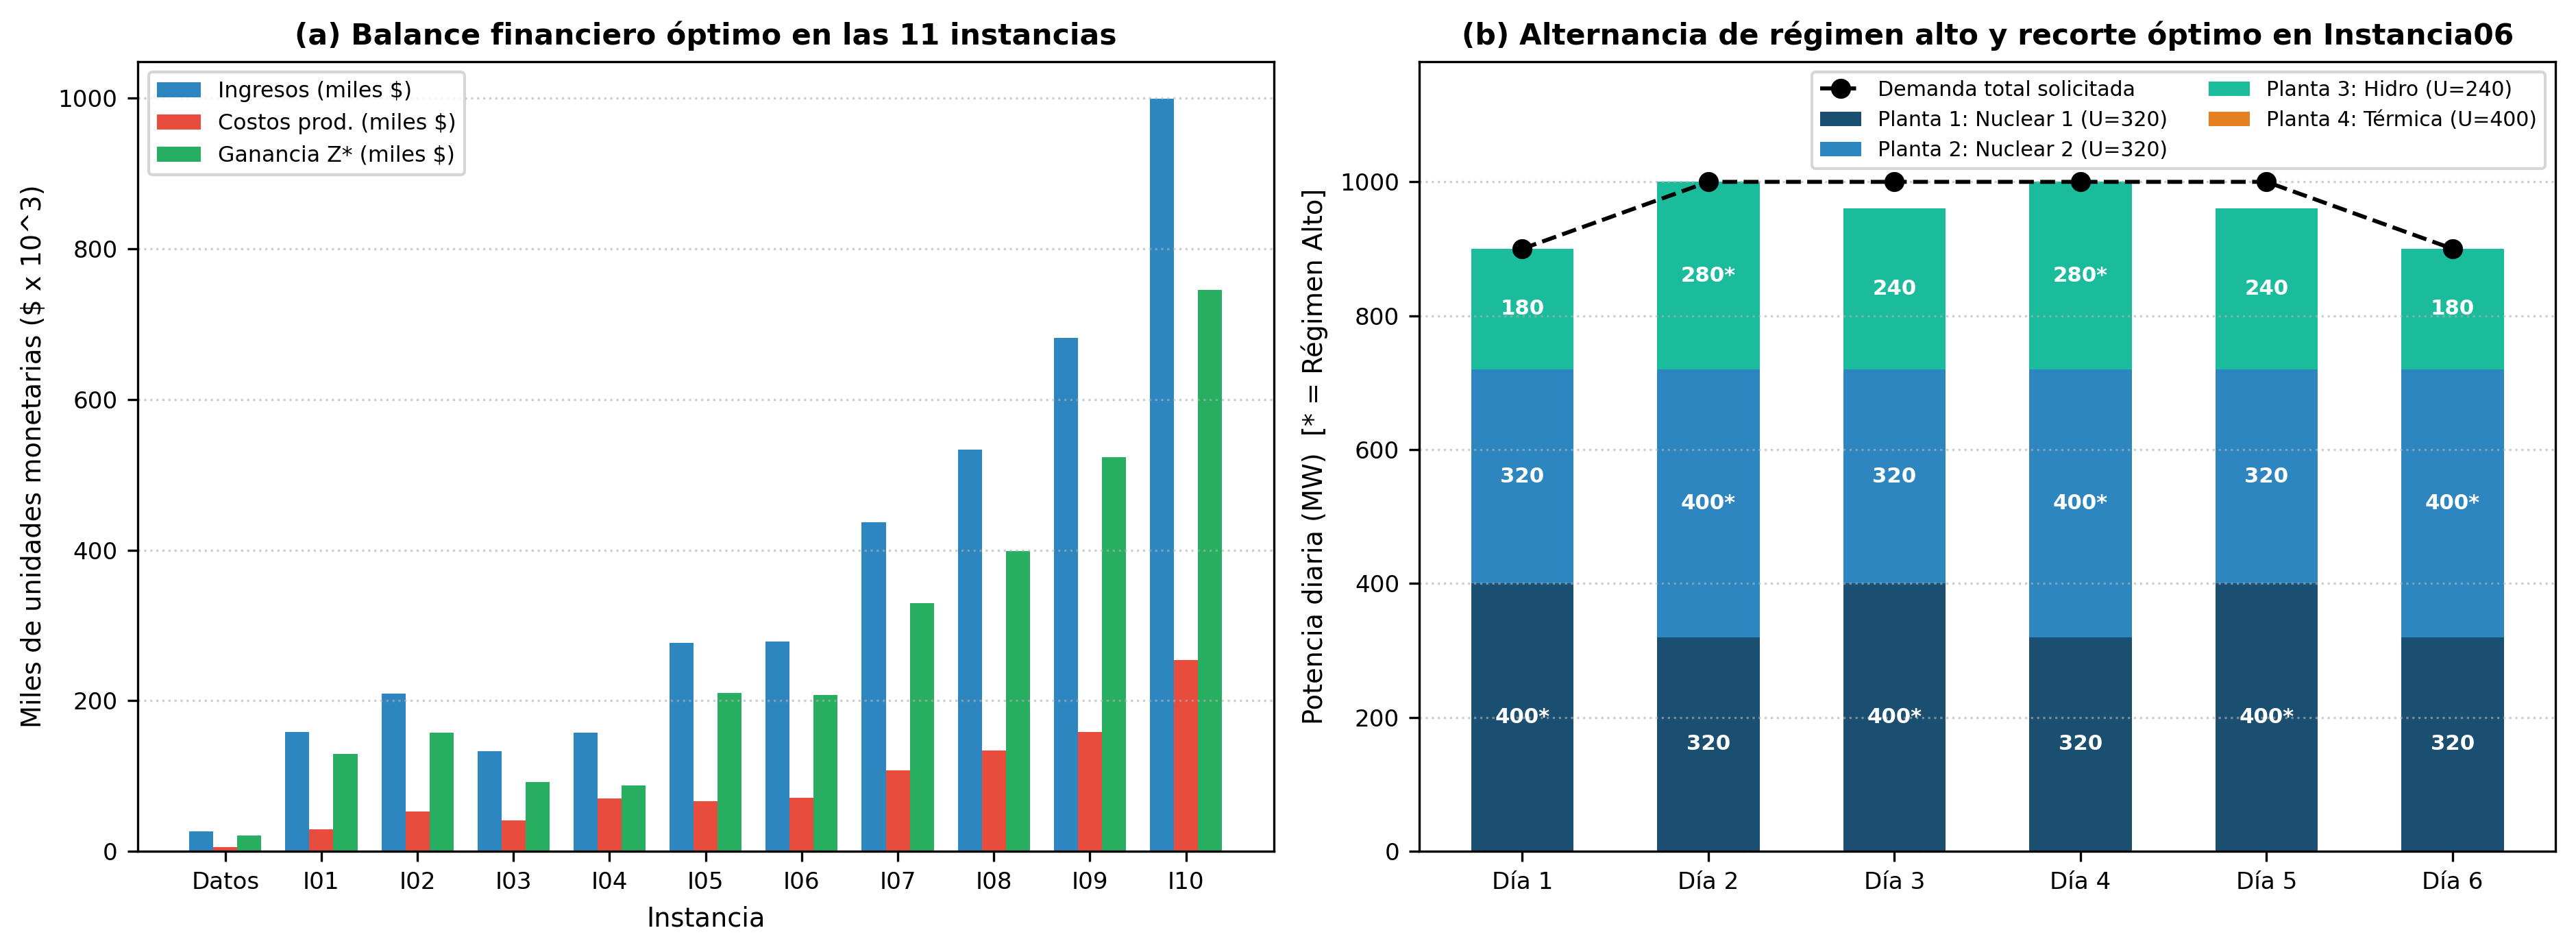
\includegraphics[width=0.98\textwidth]{1/despacho_instancias.png}
    \caption{Análisis económico-operativo de las pruebas: (a) ingresos, costos y ganancia óptima $Z^*$ en las 11 instancias; (b) despacho diario por planta en \texttt{Instancia06.dzn}, ilustrando la alternancia de régimen alto ($400^*\text{ MW}$ frente a $320\text{ MW}$) entre las dos centrales Nucleares gemelas y la Hidroeléctrica ($280^*\text{ MW}$ frente a $240\text{ MW}$).}
    \label{fig:despacho_instancias}
\end{figure}

El examen detallado de las soluciones óptimas en la Tabla~\ref{tab:resultados_instancias} y la Figura~\ref{fig:despacho_instancias}b revela tres comportamientos operativos clave:
\begin{enumerate}
    \item \textbf{Sincronización desfasada de turbinas ante la restricción de régimen alto ($C_4$):} En \texttt{Instancia06.dzn} (Figura~\ref{fig:despacho_instancias}b), las dos centrales Nucleares gemelas ($Cap_1=Cap_2=400\text{ MW}$, $U_1=U_2=320\text{ MW}$, $R_1=R_2=2$) no pueden operar dos días seguidos por encima de $320\text{ MW}$. El optimizador descubre automáticamente un patrón de relevo en contrafase: la Nuclear 1 opera en régimen alto ($400^*\text{ MW}$) en los días impares ($1, 3, 5$) y descansa exactamente en el umbral normal ($320\text{ MW}$) en los días pares ($2, 4, 6$), mientras que la Nuclear 2 descansa en $320\text{ MW}$ en los días impares y asume el régimen alto ($400^*\text{ MW}$) en los días pares. De este modo, el subparque nuclear entrega de forma constante $720\text{ MW}$ diarios a costo mínimo ($10\text{ \$/MW}$) sin infringir jamás la ventana $R_i = 2$.
    \item \textbf{Racionamiento selectivo frente a centrales de punta costosas:} En la sexta instancia (\texttt{Instancia06.dzn}), los días $2, 3, 4$ y $5$ presentan una demanda total de $1\,000\text{ MW}$. En los días $2$ y $4$, la central Hidroeléctrica ($c_3=20$, $U_3=240$, $R_3=2$) entra en régimen alto aportando $280^*\text{ MW}$ para completar los $1\,000\text{ MW}$. Sin embargo, en los días $3$ y $5$, la Hidroeléctrica está obligada a enfriarse en $240\text{ MW}$ ($720 + 240 = 960\text{ MW}$). Para cubrir los $40\text{ MW}$ restantes hacia la demanda máxima del Cliente 4 ($P_4 = 25\text{ \$/MW}$, $d_{4,3}=140$, $d^{\min}_{4,3}=70$), la única planta disponible sería la Térmica ($c_4 = 35\text{ \$/MW}$). Como $P_4 - c_4 = -10\text{ \$/MW} < 0$, el modelo mantiene apagada la Térmica ($0\text{ MW}$) y recorta en $40\text{ MW}$ la venta al Cliente 4 en los días $3$ y $5$ ($98.6\%$ de satisfacción global), ahorrando $\$800$ de pérdida operativa.
    \item \textbf{Resiliencia ante retiro de centrales:} Al eliminar la planta Nuclear en la cuarta instancia ($np=2$), las centrales Hidroeléctrica y Térmica priorizan el $100\%$ de la demanda de los Clientes 1 y 2 ($P_1=65, P_2=50 > c_T=28$) y suministran exactamente el piso legal ($G=50\%$) al Cliente 3 ($P_3=24 < c_T=28$), alcanzando $Z^* = 87\,720$ en solo $11$ nodos.
\end{enumerate}

\subsection{Análisis de Ablación: Impacto de las Restricciones Redundantes y Simetrías}

La Tabla~\ref{tab:ablacion_cop} y las Figuras~\ref{fig:arbol_bnb_cop}a y~\ref{fig:comparacion_poda_cop} cuantifican el aporte progresivo de las mejoras de modelado comparando cinco variantes acumulativas bajo la estrategia oficial $E_1$ con límite de corte de $2\,500\text{ ms}$: $M_0$ (borrador inicial con booleanas reificadas \texttt{total} y \texttt{parcial} sin redundantes), $M_1$ (modelo primario limpio $C_1$--$C_4$), $M_2$ ($M_1 + R_1 + R_2 + R_3$), $M_3$ ($M_2 + R_4 + R_5$) y $M_4$ ($M_3 + S_1 + S_2$).

\begin{table}[htbp]
    \centering
    \scriptsize
    \setlength{\tabcolsep}{1.8pt}
    \caption{Estudio de ablación ($M_0 \to M_4$): nodos explorados y propagaciones en Gecode 6.4.0 y Chuffed 0.14.0 (TO = Timeout $> 2.5\text{ s}$).}
    \label{tab:ablacion_cop}
    \begin{tabular}{lrrrrrrrr}
        \toprule
        & \multicolumn{4}{c}{Gecode 6.4.0 — Nodos (Propagaciones)} & \multicolumn{4}{c}{Chuffed 0.14.0 — Nodos (Propagaciones)} \\
        \cmidrule(lr){2-5} \cmidrule(lr){6-9}
        Instancia & $M_0 / M_1$ & $M_2$ ($+R_{1..3}$) & $M_3$ ($+R_{4..5}$) & $M_4$ ($+S_{1..2}$) & $M_0 / M_1$ & $M_2$ ($+R_{1..3}$) & $M_3$ ($+R_{4..5}$) & $M_4$ ($+S_{1..2}$) \\
        \midrule
        \texttt{Datos.dzn}       & TO & $21$ ($181$) & $1$ ($264$) & $\mathbf{1}$ ($264$) & TO & $27$ ($190$) & $1$ ($67$) & $\mathbf{1}$ ($67$) \\
        \texttt{Instancia01.dzn} & TO & $37$ ($335$) & $5$ ($464$) & $\mathbf{5}$ ($464$) & TO & $42$ ($295$) & $6$ ($161$) & $\mathbf{6}$ ($161$) \\
        \texttt{Instancia02.dzn} & TO & TO           & $48$ ($3.0\text{k}$) & $\mathbf{48}$ ($3.0\text{k}$) & TO & TO & $53$ ($1.2\text{k}$) & $\mathbf{53}$ ($1.2\text{k}$) \\
        \texttt{Instancia03.dzn} & TO & TO           & $98$ ($6.5\text{k}$) & $\mathbf{98}$ ($6.5\text{k}$) & TO & TO & $64$ ($2.4\text{k}$) & $\mathbf{64}$ ($2.4\text{k}$) \\
        \texttt{Instancia05.dzn} & TO & TO           & $199$ ($21\text{k}$) & $\mathbf{199}$ ($21\text{k}$) & TO & TO & $161$ ($12\text{k}$) & $\mathbf{161}$ ($12\text{k}$) \\
        \texttt{Instancia06.dzn} & TO & TO           & $432$ ($46\text{k}$) & $\mathbf{304}$ ($29\text{k}$) & TO & TO & $193$ ($16\text{k}$) & $\mathbf{163}$ ($13\text{k}$) \\
        \texttt{Instancia08.dzn} & TO & TO           & $3\,062$ ($481\text{k}$) & $\mathbf{3\,062}$ ($481\text{k}$) & TO & TO & $676$ ($55\text{k}$) & $\mathbf{676}$ ($55\text{k}$) \\
        \texttt{Instancia10.dzn} & TO & TO           & $143\text{k}$ ($30\text{M}$) & $\mathbf{95.8\text{k}}$ ($20\text{M}$) & TO & TO & $16.6\text{k}$ ($1.1\text{M}$) & $\mathbf{14.5\text{k}}$ ($1.2\text{M}$) \\
        \bottomrule
    \end{tabular}
\end{table}

\begin{figure}[htbp]
    \centering
    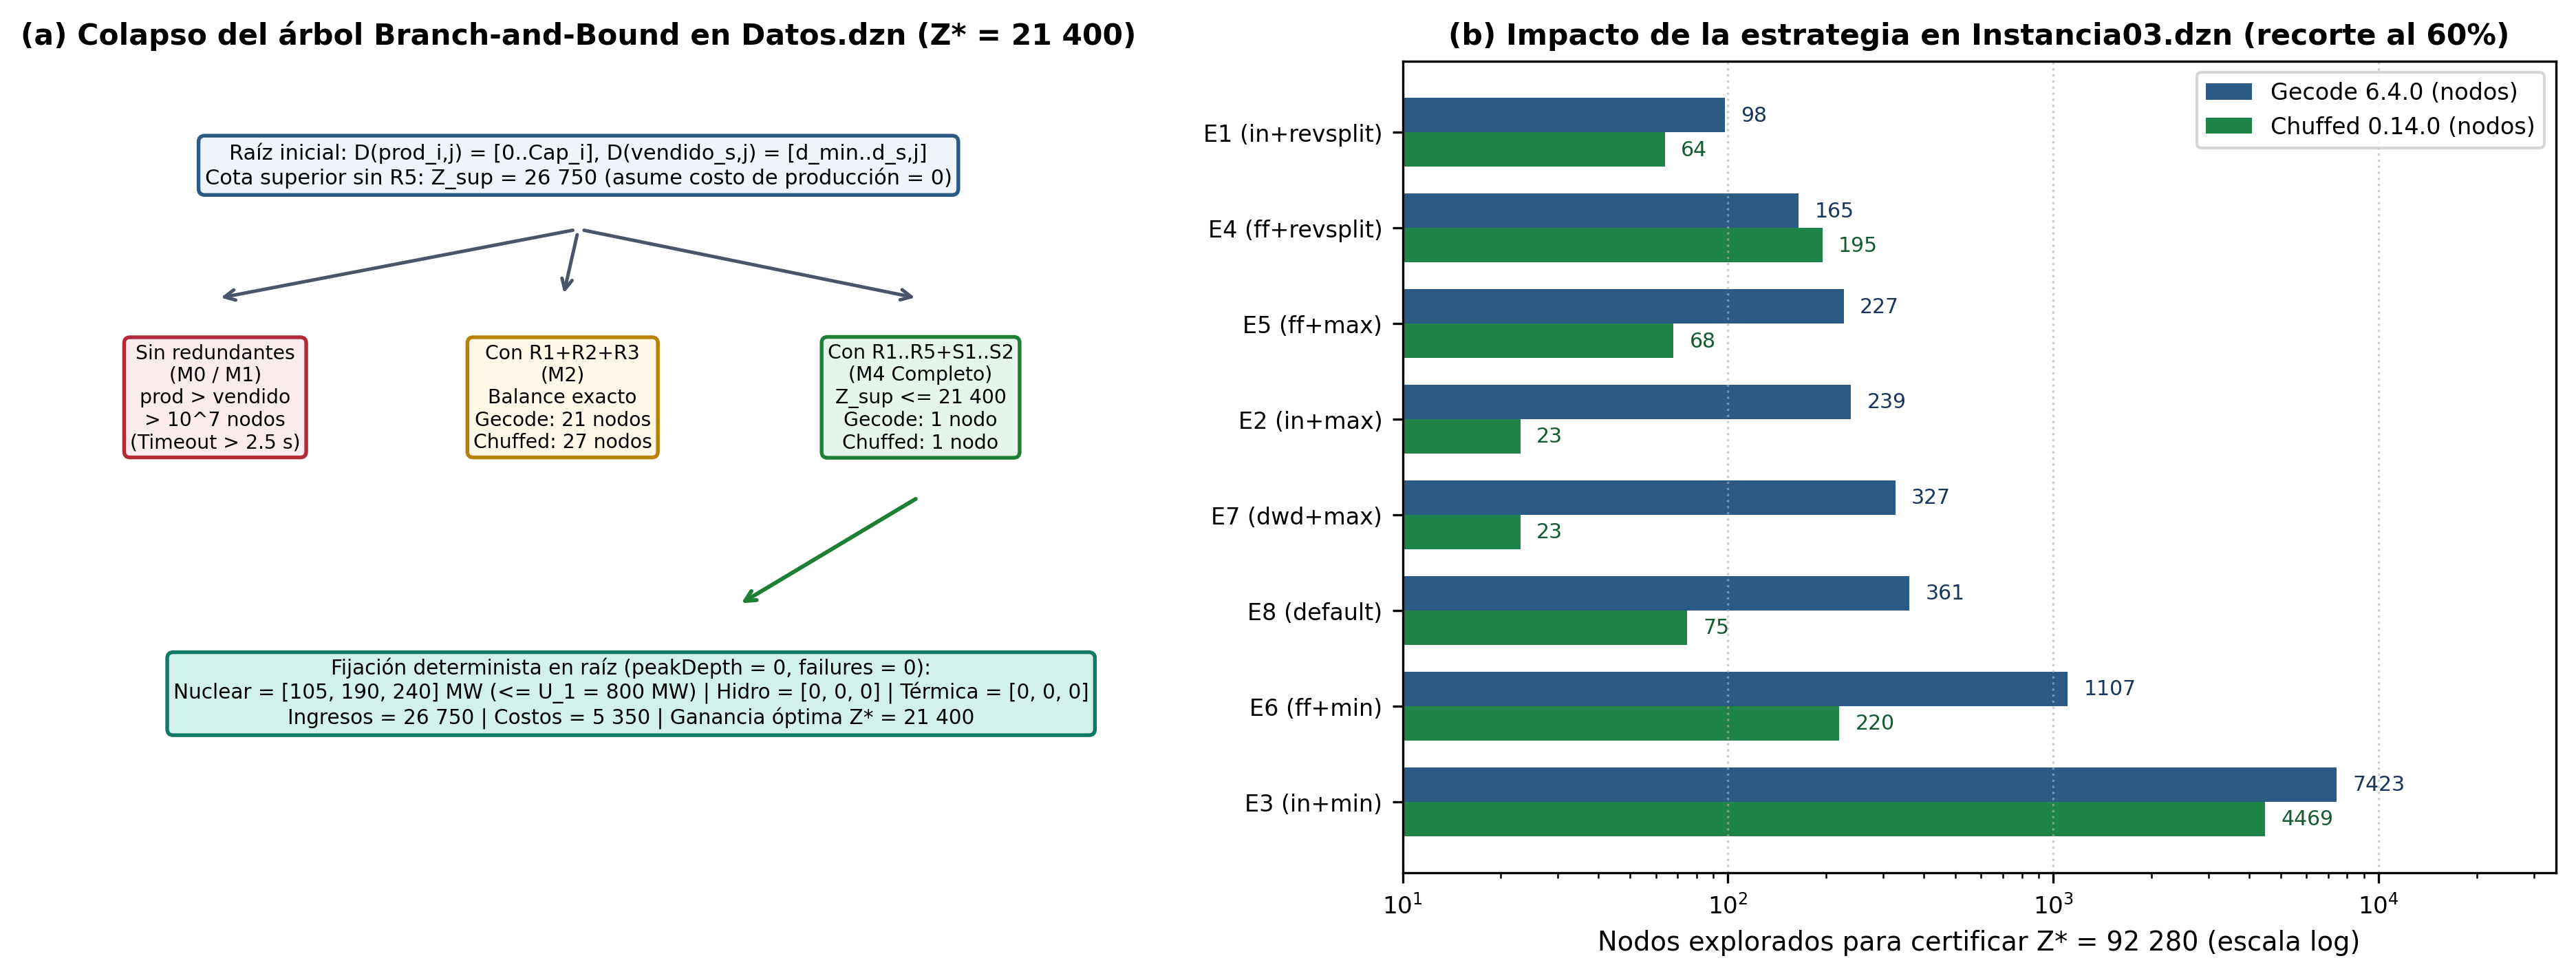
\includegraphics[width=0.98\textwidth]{1/arbol_bnb_cop.png}
    \caption{Efecto estructural de las mejoras sobre \emph{Branch-and-Bound}: (a) colapso a $1$ nodo raíz en \texttt{Datos.dzn} mediante la proyección de Fourier-Motzkin $R_5$; (b) comparación de nodos explorados por las 8 estrategias de búsqueda en \texttt{Instancia03.dzn}.}
    \label{fig:arbol_bnb_cop}
\end{figure}

\begin{figure}[htbp]
    \centering
    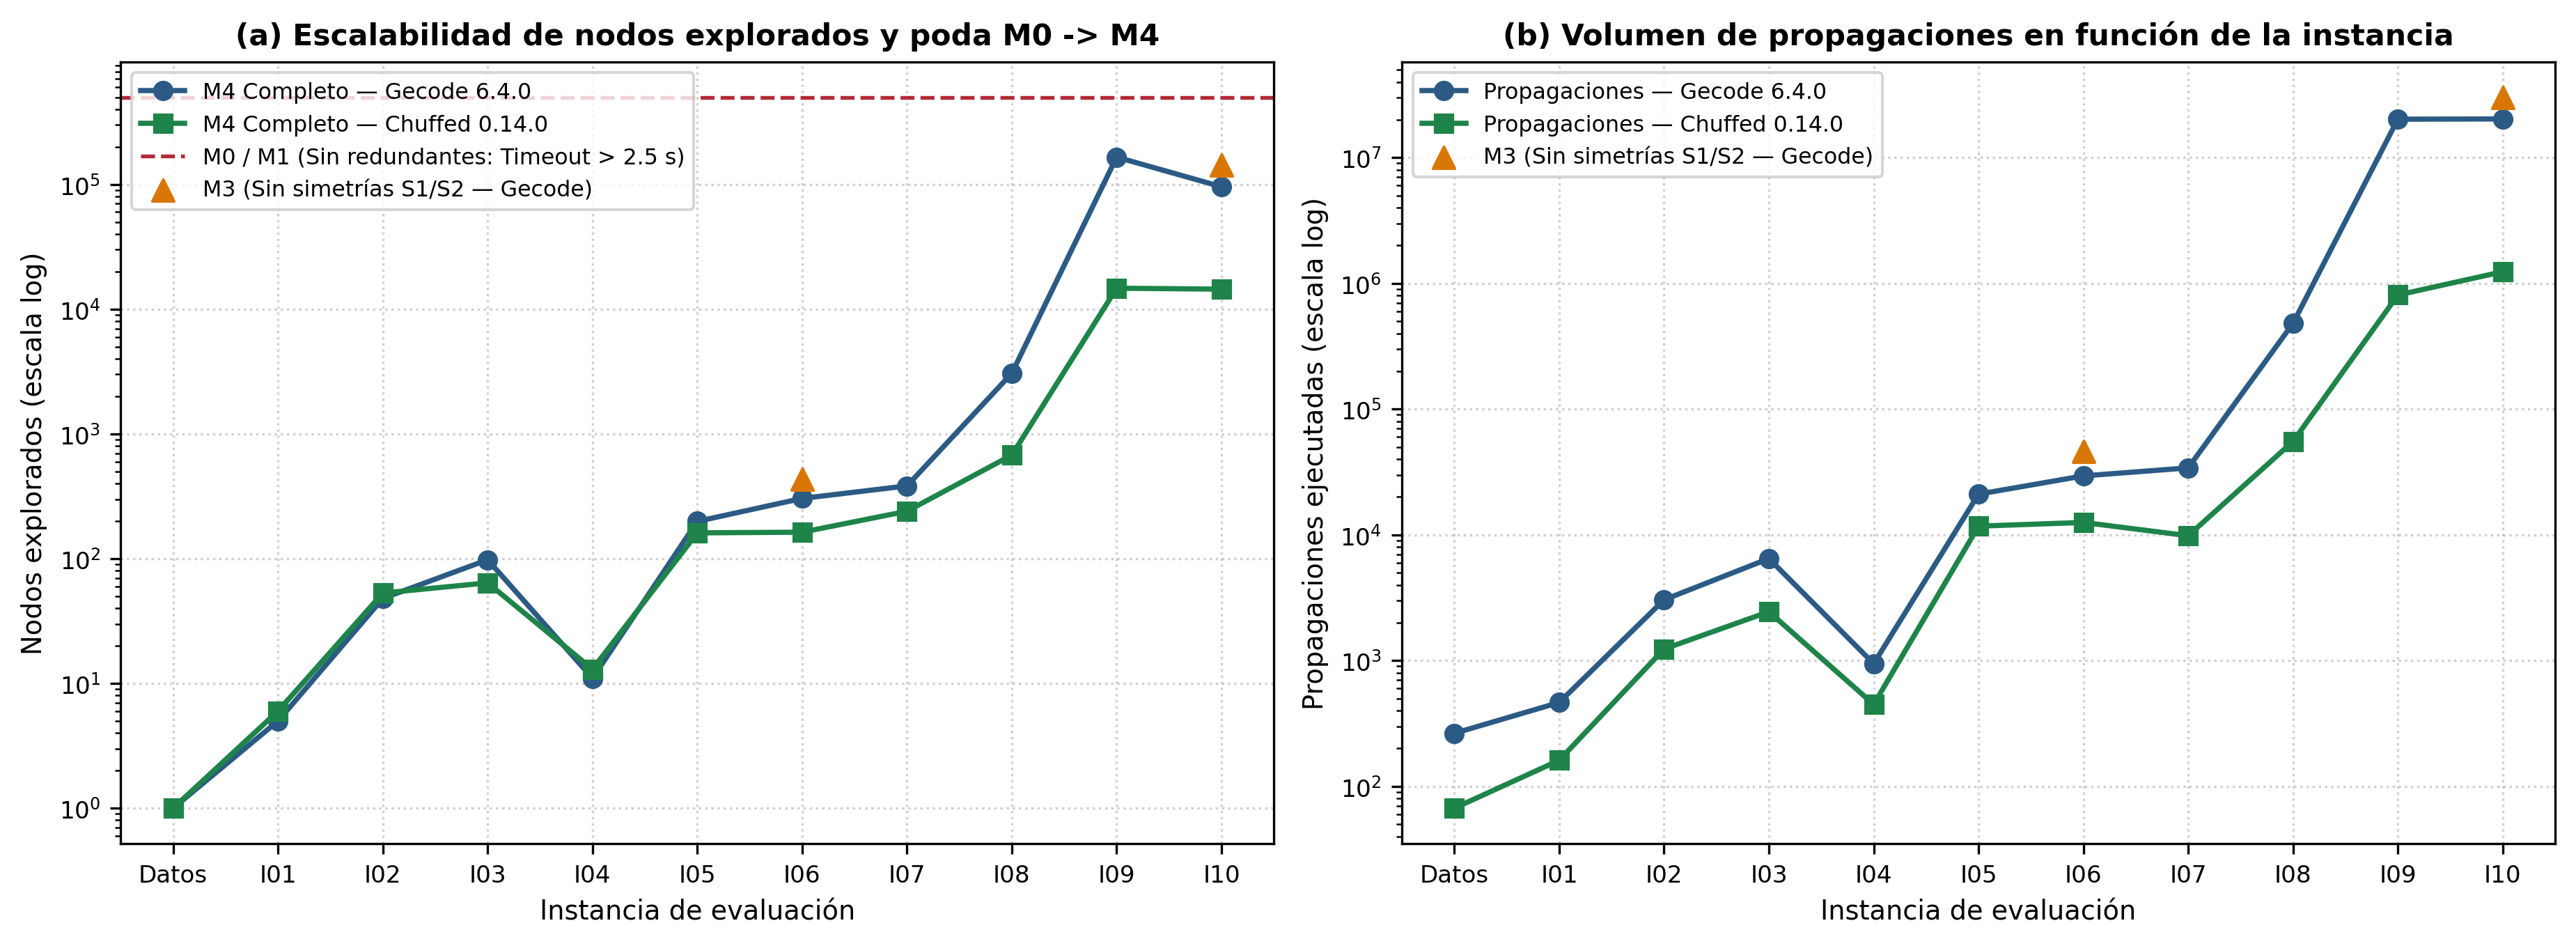
\includegraphics[width=0.98\textwidth]{1/comparacion_poda_cop.png}
    \caption{Escalabilidad del modelo completo $M_4$ frente a las variantes de ablación en las 11 instancias: (a) nodos explorados en escala logarítmica; (b) propagaciones ejecutadas por Gecode 6.4.0 y Chuffed 0.14.0.}
    \label{fig:comparacion_poda_cop}
\end{figure}

Los resultados de ablación demuestran empíricamente las propiedades teóricas deducidas en la Sección~\ref{sec:implementacion}:
\begin{itemize}
    \item \textbf{Transición de intratable ($M_0/M_1$) a resolución exacta mediante $R_1$--$R_3$ ($M_2$) y $R_4$--$R_5$ ($M_3$):} Sin la igualdad de balance diario $R_2$, tanto $M_0$ como $M_1$ exceden el tiempo límite incluso en la instancia más pequeña (\texttt{Datos.dzn}, $18$ variables), debido a la explosión combinatoria de estados con sobreproducción $\sum prod > \sum vendido$. Incorporar $R_1+R_2+R_3$ ($M_2$) resuelve \texttt{Datos.dzn} en $21$ nodos y \texttt{Instancia01.dzn} en $37$ nodos, pero resulta insuficiente cuando múltiples plantas operan en régimen alto (\texttt{Instancia02.dzn} en adelante). Al añadir la dominancia de mérito $R_4$ y las proyecciones de Fourier-Motzkin $R_5$ ($M_3$), la cota superior dual $\overline{Z}$ se cierra en el nodo raíz de \texttt{Datos.dzn} ($21 \to 1$ nodo, $0$ fallos) y permite resolver la totalidad de las 11 instancias.
    \item \textbf{Poda efectiva por rompimiento de simetrías ($M_3 \to M_4$):} En las instancias sin plantas gemelas (\texttt{Datos.dzn} a \texttt{Instancia05.dzn} e \texttt{Instancia08.dzn}), el predicado estático \texttt{where} de $S_1$ y $S_2$ se evalúa en falso durante la compilación y añade exactamente cero propagadores ($M_3 \equiv M_4$). En cambio, cuando existen plantas gemelas, $S_1$ y $S_2$ eliminan permutaciones redundantes entre filas equivalentes: en \texttt{Instancia06.dzn} (2 Nucleares gemelas) reducen los nodos de Gecode en un \textbf{$29.6\%$} ($432 \to 304$) y las propagaciones en un \textbf{$35.8\%$} ($45\,778 \to 29\,410$), mientras que en \texttt{Instancia10.dzn} (3 pares de plantas gemelas y 1 par de clientes gemelos) reducen los nodos de Gecode en un \textbf{$33.2\%$} ($143\,390 \to 95\,808$, ahorrando $9.93$ millones de propagaciones) y los de Chuffed en un \textbf{$12.8\%$} ($16\,590 \to 14\,463$).
\end{itemize}

\subsection{Comparación Experimental de las Estrategias de Búsqueda}

La Tabla~\ref{tab:estrategias_cop} y la Figura~\ref{fig:estrategias_busqueda_cop} comparan el rendimiento de las ocho estrategias de búsqueda definidas en la Sección~\ref{sec:busqueda} aplicadas sobre el modelo completo $M_4$.

\begin{table}[htbp]
    \centering
    \scriptsize
    \setlength{\tabcolsep}{0.9pt}
    \caption{Comparación estadística de las 8 estrategias de búsqueda sobre el modelo completo $M_4$ (TO = Timeout $> 2.5\text{ s}$).}
    \label{tab:estrategias_cop}
    \begin{tabular}{llrrrrrrrrrr}
        \toprule
        & & \multicolumn{5}{c}{Gecode 6.4.0 — Nodos ($t_{\text{solve}}$ ms)} & \multicolumn{5}{c}{Chuffed 0.14.0 — Nodos ($t_{\text{solve}}$ ms)} \\
        \cmidrule(lr){3-7} \cmidrule(lr){8-12}
        Cód. & Estrategia & \texttt{I02} & \texttt{I03} & \texttt{I06} & \texttt{I08} & \texttt{I10} & \texttt{I02} & \texttt{I03} & \texttt{I06} & \texttt{I08} & \texttt{I10} \\
        \midrule
        $E_1$ & \texttt{in,revsplit} & $48$ ($0.3$) & $\mathbf{98}$ ($\mathbf{0.6}$) & $\mathbf{304}$ ($\mathbf{2.1}$) & $\mathbf{3.1\text{k}}$ ($\mathbf{40}$) & $\mathbf{96\text{k}}$ ($\mathbf{1.5\text{s}}$) & $53$ ($1$) & $64$ ($1$) & $163$ ($3$) & $676$ ($14$) & $14\text{k}$ ($\mathbf{473}$) \\
        $E_2$ & \texttt{in,max}      & $\mathbf{8}$ ($\mathbf{0.1}$) & $239$ ($1.1$) & $1.4\text{k}$ ($6.1$) & $53\text{k}$ ($425$) & TO & $\mathbf{13}$ ($\mathbf{0}$) & $\mathbf{23}$ ($\mathbf{0}$) & $\mathbf{64}$ ($\mathbf{2}$) & $\mathbf{284}$ ($\mathbf{13}$) & $12\text{k}$ ($623$) \\
        $E_3$ & \texttt{in,min}      & $7.8\text{k}$ ($16$) & $7.4\text{k}$ ($17$) & $29\text{k}$ ($69$) & $303\text{k}$ ($2.0\text{s}$) & TO & $4.0\text{k}$ ($27$) & $4.5\text{k}$ ($34$) & $23\text{k}$ ($174$) & $89\text{k}$ ($868$) & TO \\
        $E_4$ & \texttt{ff,revsplit} & $69$ ($0.4$) & $165$ ($1.2$) & $3.1\text{k}$ ($12$) & $6.0\text{k}$ ($42$) & TO & $69$ ($1$) & $195$ ($3$) & $1.2\text{k}$ ($12$) & $828$ ($45$) & TO \\
        $E_5$ & \texttt{ff,max}      & $135$ ($0.6$) & $227$ ($0.8$) & $2.4\text{k}$ ($8.0$) & $24\text{k}$ ($123$) & TO & $389$ ($7$) & $68$ ($2$) & $659$ ($18$) & $1.5\text{k}$ ($88$) & TO \\
        $E_6$ & \texttt{ff,min}      & $2.8\text{k}$ ($4.9$) & $1.1\text{k}$ ($3.3$) & $8.9\text{k}$ ($28$) & $237\text{k}$ ($817$) & TO & $2.2\text{k}$ ($17$) & $220$ ($5$) & $1.1\text{k}$ ($31$) & $4.2\text{k}$ ($296$) & TO \\
        $E_7$ & \texttt{dwd,max}     & $15$ ($0.2$) & $327$ ($1.1$) & $1.0\text{k}$ ($4.2$) & $12\text{k}$ ($82$) & TO & $\mathbf{13}$ ($\mathbf{0}$) & $\mathbf{23}$ ($1$) & $\mathbf{64}$ ($5$) & $\mathbf{284}$ ($15$) & $12\text{k}$ ($568$) \\
        $E_8$ & \texttt{default}     & $1.7\text{k}$ ($3.1$) & $361$ ($1.2$) & $3.4\text{k}$ ($8.3$) & $39\text{k}$ ($235$) & TO & $102$ ($2$) & $75$ ($2$) & $190$ ($8$) & $534$ ($36$) & $\mathbf{4.0\text{k}}$ ($535$) \\
        \bottomrule
    \end{tabular}
\end{table}

\begin{figure}[htbp]
    \centering
    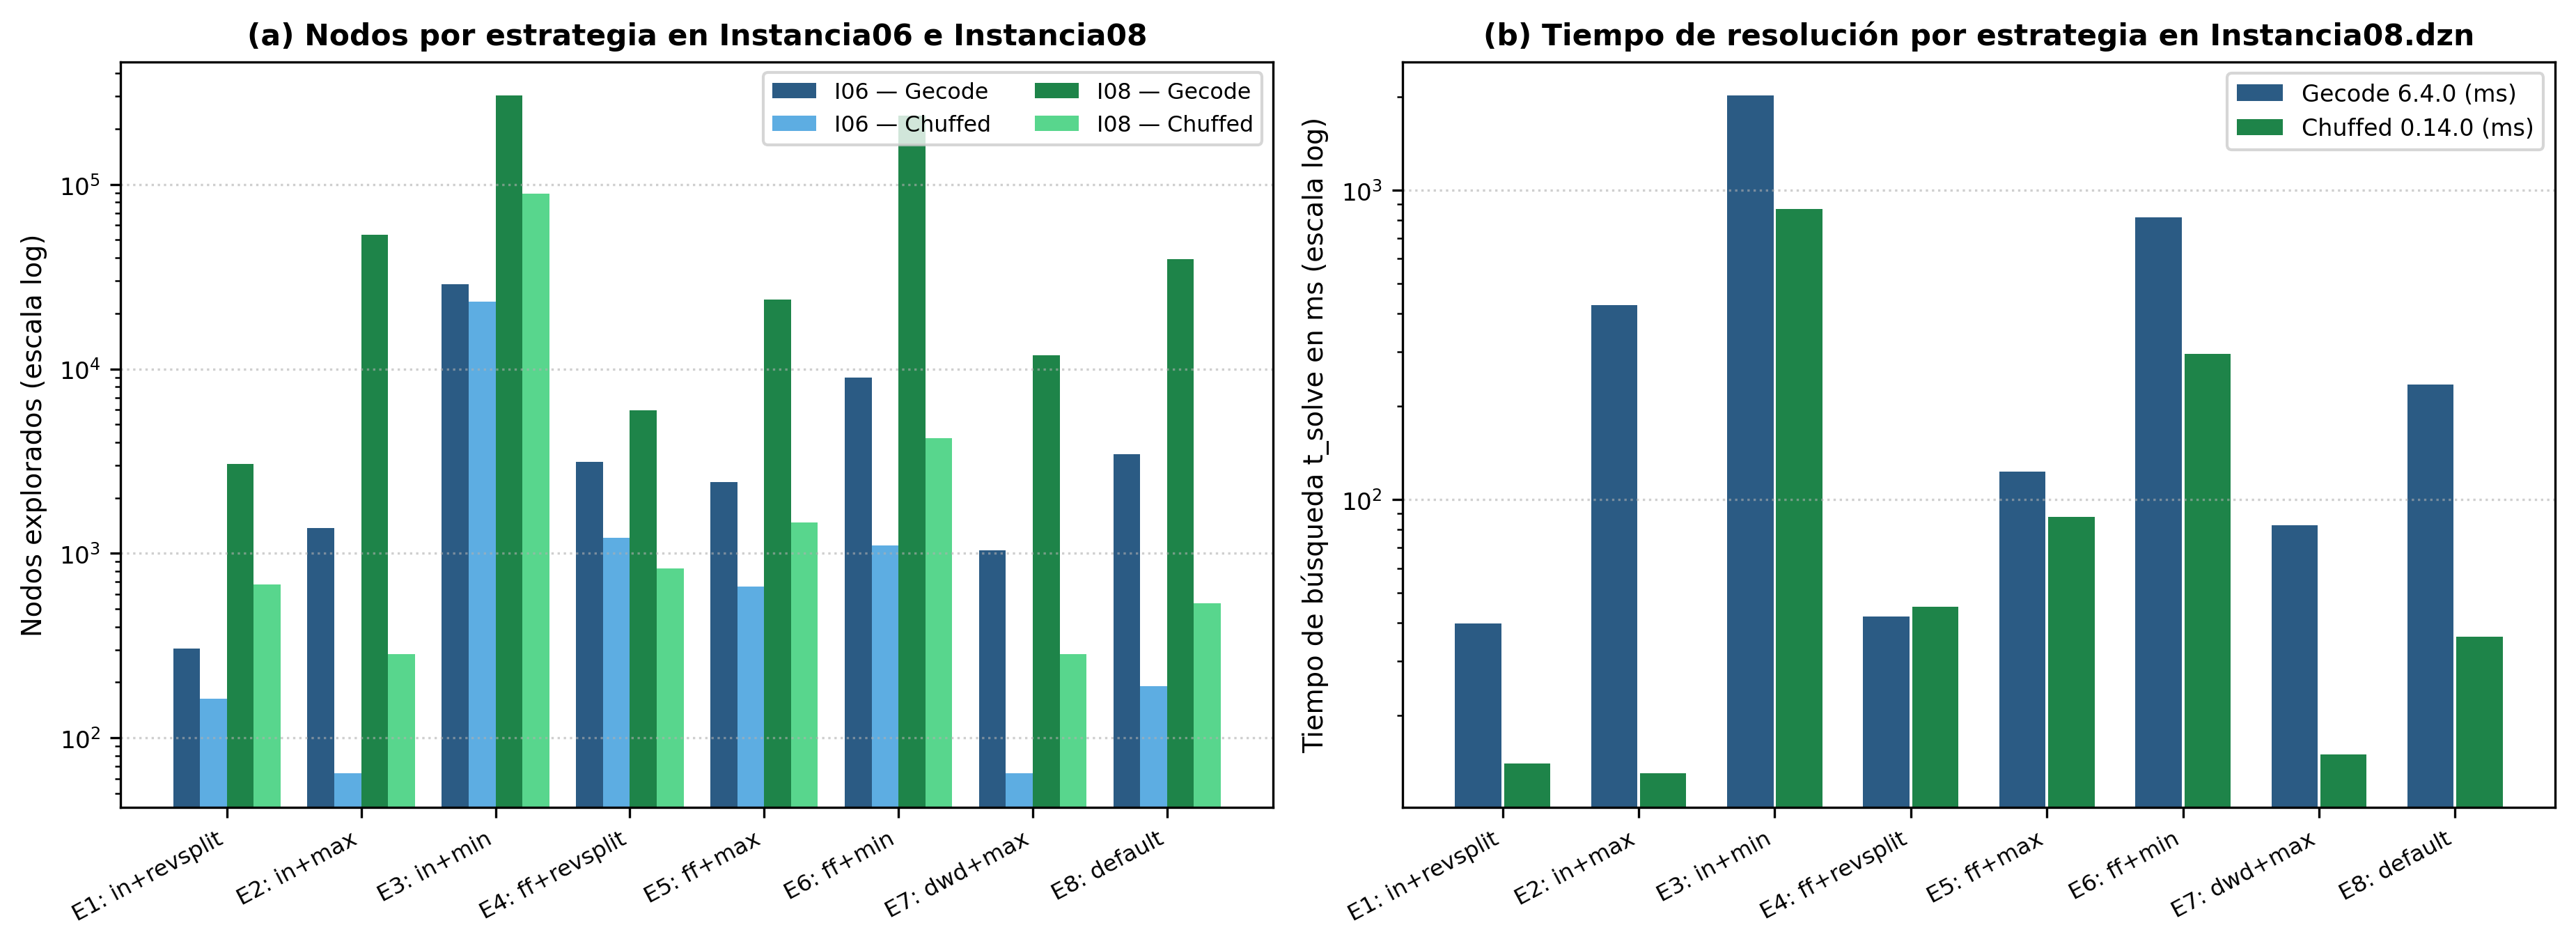
\includegraphics[width=0.98\textwidth]{1/estrategias_busqueda_cop.png}
    \caption{Desempeño comparativo de las 8 estrategias de búsqueda ($E_1$--$E_8$): (a) nodos explorados en \texttt{Instancia06.dzn} e \texttt{Instancia08.dzn}; (b) tiempos de resolución $t_{\text{solve}}$ (ms) en \texttt{Instancia08.dzn}.}
    \label{fig:estrategias_busqueda_cop}
\end{figure}

La evidencia experimental de la Tabla~\ref{tab:estrategias_cop} y la Figura~\ref{fig:estrategias_busqueda_cop} confirma de forma contundente la teoría expuesta en la Sección~\ref{subsec:teoria_busqueda}:
\begin{itemize}
    \item \textbf{Robustez y escalabilidad superior de $E_1$ (orden de entrada con bisección descendente):} $E_1$ es la \textbf{única estrategia de las ocho evaluadas} capaz de resolver la totalidad de las 11 instancias hasta optimalidad certificada dentro del límite de tiempo en ambos motores (\texttt{Instancia10.dzn}: $95\,808$ nodos y $1.48\text{ s}$ en Gecode; $14\,463$ nodos y $0.47\text{ s}$ en Chuffed). En \texttt{Instancia08.dzn} bajo Gecode, $E_1$ ($3\,062$ nodos, $39.8\text{ ms}$) reduce los nodos en un factor de \textbf{$17.4\times$} frente a la enumeración unitaria descendente $E_2$ ($53\,167$ nodos, $425.5\text{ ms}$), en \textbf{$12.8\times$} frente a la búsqueda por defecto $E_8$ ($39\,337$ nodos), en \textbf{$77.3\times$} frente a la estrategia del borrador inicial $E_6$ ($236\,811$ nodos) y en \textbf{$99.0\times$} frente a $E_3$ ($303\,157$ nodos, $2\,022.6\text{ ms}$).
    \item \textbf{Ventaja de \texttt{input\_order} ($prod \to vendido$) frente a \texttt{first\_fail}:} Comparando a igualdad de selector de valor ($E_1$ frente a $E_4$, y $E_2$ frente a $E_5$), \texttt{input\_order} supera sistemáticamente a \texttt{first\_fail} en \texttt{Instancia06.dzn} ($304$ frente a $3\,128$ nodos en Gecode; $163$ frente a $1\,219$ en Chuffed) y en \texttt{Instancia10.dzn} (donde todas las variantes con \texttt{first\_fail}, $E_4$--$E_6$, sufren \emph{timeout} en ambos motores). Ello verifica que preservar el orden causal de decisión (primero la trayectoria de las centrales por orden de mérito y después la asignación comercial a clientes) evita ramificar prematuramente sobre los dominios estrechos de $vendido_{s,j}$.
    \item \textbf{Sinergia entre aprendizaje de cláusulas (Chuffed) y selección de valor máximo ($E_2, E_7$):} Mientras que Gecode requiere bisección de intervalos ($E_1$) para no degradarse en escalones de capacidad grandes, Chuffed representa internamente los enteros mediante literales booleanos de cota $[\![ x \le v ]\!]$ y aprende cláusulas de conflicto (\emph{nogoods}) que saltan directamente desde $Cap_i$ hasta el umbral $U_i$ en un solo \emph{backjump}. Gracias a ello, en Chuffed las estrategias $E_2$ y $E_7$ resuelven \texttt{Instancia03.dzn}, \texttt{Instancia06.dzn} e \texttt{Instancia08.dzn} en apenas $23$, $64$ y $284$ nodos respectivamente.
\end{itemize}

\newpage

% !TEX root = ../main.tex
\section{Conclusiones}
\label{sec:conclusiones}

A partir del desarrollo formal, la implementación declarativa en MiniZinc y la evaluación experimental sobre el caso base y las diez instancias de planificación energética, se establecen las siguientes conclusiones técnicas justificadas por los resultados obtenidos:

\begin{enumerate}
    \item \textbf{Importancia crítica del acoplamiento dual en la función objetivo de un COP lineal entero:}
    En problemas de optimización donde la función objetivo maximiza la diferencia entre ingresos comerciales y costos de producción ($Z = \sum P_s vendido_{s,j} - \sum c_i prod_{i,j}$), la formulación primaria por sí sola presenta una relajación de intervalos débil, pues el propagador de la ecuación objetivo evalúa el máximo ingreso asumiendo simultáneamente producción nula ($\underline{prod}_{i,j} = 0$). La incorporación de la igualdad de flujo diario sin sobreproducción estéril ($R_2$), la dominancia por orden de mérito a través de la frontera de régimen normal ($R_4$) y las proyecciones lineales por escalón de costo marginal ($R_5$) acopló algebraicamente el costo mínimo de generación al margen neto por megavatio vendido $(P_s - c_q)$. Como se demostró en la Tabla~\ref{tab:ablacion_cop}, esta reformulación transformó un modelo que sufría \emph{timeout} ($>2.5\text{ s}$) incluso en $18$ variables ($M_0/M_1$) en un modelo que resuelve \texttt{Datos.dzn} determinísticamente en el nodo raíz ($1$ nodo, $0$ fallos, $0.09\text{ ms}$) y escala hasta instancias de $168$ variables con tres pares de plantas gemelas (\texttt{Instancia10.dzn}).

    \item \textbf{Generalidad estructural y exactitud de la restricción de régimen alto en todo el parque:}
    La corrección de la ventana deslizante de longitud exacta $R_i$ días ($k \in \{1, \dots, n - R_i + 1\}$ con $d \in \{0, \dots, R_i - 1\}$) aplicada uniformemente a todas las centrales eléctricas $i \in P$, complementada por la cota lineal acumulada por ventana $R_3$ \eqref{eq:r3_ventana_lineal}, permitió capturar con fidelidad el desgaste diferencial de turbinas nucleares, hidroeléctricas, térmicas y renovables. Los experimentos en \texttt{Instancia02.dzn} e \texttt{Instancia06.dzn} evidenciaron que el modelo planifica automáticamente esquemas de alternancia en contrafase entre centrales (operando un día a capacidad nominal $Cap_i$ en régimen alto y enfriando la turbina al día siguiente exactamente en su umbral normal $U_i$), y que cuando el costo marginal de la central de respaldo supera la tarifa de un cliente ($P_s < c_i$ en \texttt{Instancia03.dzn}, \texttt{Instancia04.dzn}, \texttt{Instancia06.dzn}, \texttt{Instancia08.dzn} e \texttt{Instancia10.dzn}), recorta de manera óptima la entrega de dicho cliente hacia su piso garantizado $G\%$ para evitar pérdidas operativas.

    \item \textbf{Eficacia del rompimiento de simetrías en parques con unidades modulares equivalentes:}
    El análisis de simetrías demostró que estás sólo existen dos o más centrales comparten idéntica tripla $(c_i, Cap_i, R_i)$ o cuando dos clientes comparten tarifa y perfil de demanda. La imposición de restricciones globales \texttt{lex\_greatereq} ($S_1$ y $S_2$) junto con el desempate canónico intra-día eliminó las particiones equivalentes de carga sin introducir sobrecosto en instancias heterogéneas, logrando en Gecode una reducción del $29.6\%$ de los nodos en \texttt{Instancia06.dzn} ($432 \to 304$) y del $33.2\%$ en \texttt{Instancia10.dzn} ($143\,390 \to 95\,808$ nodos y $9.93\times 10^6$ propagaciones ahorradas).

    \item \textbf{Superioridad del orden causal de decisión y la bisección descendente de intervalos:}
    El estudio comparativo de ocho estrategias de búsqueda (Tabla~\ref{tab:estrategias_cop}) refutó la idoneidad ingenua de la heurística clásica \texttt{first\_fail} + \texttt{indomain\_min} ($E_6$) para este COP: por una parte, la asimetría de escalas entre los dominios estrechos de $vendido_{s,j}$ y los dominios amplios de $prod_{i,j}$ hace que \texttt{first\_fail} ramifique sobre las ventas antes de resolver el cuello de botella inter-temporal de las plantas. Por otra parte, \texttt{indomain\_min} explora primero las asignaciones de peor ganancia ($\underline{Z}$), anulando la poda de \emph{Branch-and-Bound}. La estrategia adoptada $E_1$ (\texttt{input\_order} sobre $prod \mathbin{+\!+} vendido$ con \texttt{indomain\_reverse\_split}) resolvió la totalidad de las 11 instancias en ambos solvers, reduciendo en \texttt{Instancia08.dzn} los nodos explorados por Gecode en $17.4\times$ respecto a \texttt{indomain\_max} ($E_2$), en $77.3\times$ respecto a $E_6$ y en $99.0\times$ respecto a \texttt{indomain\_min} ($E_3$).

    \item \textbf{Validación de utilidad de técnica de generalidad:} De forma general la implementación del problema validó la gran utilidad y flexibilidad de solución que aporta la generalización de problemas de opmtimización por medio de la parametrización. Permitiendo en este caso construir un conjunto de restricciones que se adaptan a una familia de problemas de gran alta variedad como evidencian las pruebas realizadas. 
\end{enumerate}


\end{document}
